% ============================================================
% TRACE: Trust-Aware Routing and Adversarial Credit Evaluation
%        for Autonomous Agent Marketplaces
%
% Conference Workshop Draft -- ACM sigconf format (nonacm)
% Build: pdflatex -> pdflatex -> pdflatex
% ============================================================

\documentclass[sigconf,nonacm,10pt]{acmart}

% acmart already loads: amsmath, amsthm, amssymb, hyperref,
% graphicx, booktabs, xcolor, caption, microtype, etc.
% Loading them again would cause clashes (e.g. \Bbbk redefinition
% by amssymb against newtxmath shipped with acmart).

% -------------------------------------------------------------
% Additional packages that acmart does NOT preload
% -------------------------------------------------------------
\usepackage{multirow}
\usepackage{tabularx}
\usepackage{array}
\usepackage{subcaption}
\usepackage{float}
\usepackage[ruled,vlined,linesnumbered]{algorithm2e}
\usepackage{enumitem}

% -------------------------------------------------------------
% Small inline social icon helper.  We embed self-rendered
% vector icons (icon_linkedin.pdf, icon_github.pdf) via
% \includegraphics so any PDF viewer displays them
% reliably---FontAwesome's custom-encoded glyphs render as
% boxed garbage (e.g. "ï §") in some readers.
% -------------------------------------------------------------
\newcommand{\socialicon}[1]{%
  \raisebox{-0.18em}{\includegraphics[height=0.95em]{#1}}}
\newcommand{\faLinkedinPdf}{\socialicon{icon_linkedin.pdf}}
\newcommand{\faGithubPdf}{\socialicon{icon_github.pdf}}

% -------------------------------------------------------------
% Math operators
% -------------------------------------------------------------
\DeclareMathOperator*{\argmax}{arg\,max}
\DeclareMathOperator*{\argmin}{arg\,min}

% -------------------------------------------------------------
% Hyperlink colour overrides (acmart sets coloured links)
% -------------------------------------------------------------
\hypersetup{colorlinks=true,linkcolor=black,citecolor=black,urlcolor=blue}

% -------------------------------------------------------------
% Typesetting tolerances
% Allow some flexibility in justification to reduce overfull
% boxes from long technical phrases without resorting to ragged
% setting.  These values are conservative.
% -------------------------------------------------------------
\setlength{\emergencystretch}{2em}
\tolerance=1500
\hbadness=10000  % suppress underfull-hbox warnings (cosmetic)
\vbadness=10000  % suppress underfull-vbox warnings (cosmetic)

% -------------------------------------------------------------
% Increase header height to silence fancyhdr complaints from
% acmart's running head (libertine ascenders need >= 14pt; we
% use 20pt to provide a margin across the balance pass).
% -------------------------------------------------------------
\setlength{\headheight}{20pt}

% -------------------------------------------------------------
% Disable acmart's automatic \balance call.  The default behaviour
% balances the two columns of the last page using the `balance'
% package, which warns when invoked from the second column (an
% unavoidable side effect of an appendix that ends on column~2).
% Disabling it leaves the final page slightly unbalanced---an
% acceptable tradeoff for a clean log.
% -------------------------------------------------------------
\AtBeginDocument{\let\balance\relax}

% -------------------------------------------------------------
% Suppress ACM reference / copyright (workshop/preprint draft)
% -------------------------------------------------------------
\settopmatter{printacmref=false,printccs=false,printfolios=true}
\renewcommand\footnotetextcopyrightpermission[1]{}
\pagestyle{plain}

% -------------------------------------------------------------
% Figure path
% -------------------------------------------------------------
\graphicspath{{figures/}}

% =============================================================
\begin{document}

\title[TRACE for Autonomous Agent Marketplaces]{%
  TRACE: Trust-Aware Routing and Adversarial Credit Evaluation
  for Autonomous Agent Marketplaces}

\author{Nikunj Kaushik}
\affiliation{%
  \institution{%
    \href{https://www.linkedin.com/in/nikunjkaushik2005}{\faLinkedinPdf}\;%
    \href{https://github.com/NikunjKaushik20}{\faGithubPdf}%
  }
  \city{}
  \country{}
}
\email{nikunjkaushik28@gmail.com}

\author{Siddhanth Gupta}
\affiliation{%
  \institution{%
    \href{https://www.linkedin.com/in/siddhanthgupta501}{\faLinkedinPdf}\;%
    \href{https://github.com/Siddhanthguptaa}{\faGithubPdf}%
  }
  \city{}
  \country{}
}
\email{siddhanthgupta501@gmail.com}

\author{Sarthak Vashisht}
\affiliation{%
  \institution{%
    \href{https://www.linkedin.com/in/sarthakvashisht2005}{\faLinkedinPdf}\;%
    \href{https://github.com/prometheus0028}{\faGithubPdf}%
  }
  \city{}
  \country{}
}
\email{sarthak.05v@gmail.com}

\renewcommand{\shortauthors}{Kaushik, Gupta, and Vashisht}

% =============================================================
\begin{abstract}
Autonomous agent marketplaces that settle economic interactions
over payment-channel networks introduce trust challenges distinct
from classical peer-to-peer reputation settings: providers are
pseudonymous, interactions are economically settled in real time,
and adversarial agents can exploit accumulated trust histories
rather than simply inject false identities. We present
\textbf{TRACE} (\underline{T}rust-Aware \underline{R}outing and
\underline{A}dversarial \underline{C}redit \underline{E}valuation),
a trust-scoring and routing framework for payment-settled agent
marketplaces, instantiated here with Lightning payments and validated
on a live deployed pilot marketplace. TRACE~v2.1 evaluates
provider agents along four dimensions---historical task completion,
repayment and default behaviour, trust-graph topology, and
repeated-interaction decay---and routes tasks via a trust-aware
economic utility function rather than price-only or naive
reputation selection.

We evaluate TRACE under four adversarial profiles---collusion ring,
strategic default, Sybil cluster, and whitewashing---across network
sizes $N \in \{30, 50, 100, 500\}$ using 20-seed multi-seed
experiments at primary scale and a high-power $N{=}500$ replication.
Under collusion ring attack at $N{=}50$, TRACE reduces mean fraud
exposure to $43.8 \pm 23.8$~sats versus $116.0 \pm 20.8$~sats for
price-only routing (Mann--Whitney $p \approx 0.000$, Cliff's
$|\delta| = 0.976$, large effect). TRACE fraud exposure scales
favourably with network size, decreasing from $56.0$~sats at
$N{=}30$ to $9.0$~sats at $N{=}100$ ($p < 0.001$,
$|\delta| = 1.00$). Against strategic-default attack, TRACE reduces
malicious routing by approximately $1.5\times$ relative to
reputation-only routing.

A central empirical finding is negative: two architectural
extensions (v2.2, v2.3) that add adaptive penalty scaling, causal
graph failure tracking, and temporal trust dynamics produce
\emph{no statistically significant improvement} across 30~pairwise
tests, while increasing fraud variance by up to 17\% (collusion
ring, $\sigma$ from v2.1 to v2.3) and reducing honest-agent routing
share by approximately 2.5~percentage points. We propose a Bayesian
trust extension that replaces frequentist completion-rate estimation
with a Beta-posterior estimate, providing principled cold-start
handling without additional heuristics. A pilot deployment on
satsrouter.live ($35$~registered providers, $24$~completed jobs)
confirms that the TRACE implementation operates correctly in
production and that trust-score distributions on live interactions
are consistent with simulation predictions.
\end{abstract}

\keywords{autonomous agent marketplace; trust-aware routing;
  adversarial robustness; Lightning Network; reputation systems;
  collusion detection; false suppression; Sybil resistance}

\maketitle

% =============================================================
\section{Introduction}
\label{sec:intro}

The emergence of autonomous software agents that can discover,
contract, and pay for services from one another over open networks
creates a new class of economic infrastructure. Agent orchestrators
must select providers from a pool of pseudonymous participants,
compensate them via micropayment rails, and detect misbehaviour
without a central authority. The Lightning
Network~\cite{poon2016lightning}---a payment-channel system
providing near-instant, low-fee settlement---offers a practical
payment layer for such interactions. However, payment settlement
alone does not establish provider trustworthiness; adversarial
agents can collect payment without delivering contracted service,
form coordinated coalitions to inflate apparent reputation, or
register and discard identities to escape accumulated penalties.

Two seemingly natural routing strategies fail systematically under
adversarial conditions. \emph{Price-only} routing, which selects
the cheapest available provider without consulting interaction
history, offers no defence against reputation-based attacks: under
collusion ring attack ($N{=}50$, 30\% malicious agents,
20~seeds), price-only routing routes $57.4\%$ of jobs to malicious
agents and incurs $116.0$~sats of mean fraud exposure.
\emph{Reputation-only} routing, which selects the
highest-cumulative-success-rate provider, reduces collusion
exposure substantially but is structurally blind to strategic
default: agents that build legitimate histories before selectively
defaulting on high-value jobs produce more than an order of
magnitude greater fraud than a routing system aware of structural
trust patterns. Neither baseline provides adversarial robustness
across the full attack landscape.

Classical distributed trust systems address related problems but
under different assumptions.
EigenTrust~\cite{kamvar2003eigentrust} requires globally trusted
seed nodes unavailable in permissionless settings.
SybilGuard~\cite{yu2006sybilguard} and
SybilLimit~\cite{yu2008sybillimit} rely on pre-existing social
graphs absent in agent marketplaces. Reputation-only routing
accumulates success rates but provides no structural defence
against agents that \emph{exploit} accumulated reputation to
default selectively---the very pattern Dellarocas identified as
the principal failure mode of accumulated-history reputation
systems in early online platforms~\cite{dellarocas2003digitization}.

\noindent\textbf{This paper.}
We present \textbf{TRACE~v2.1}, a composite trust-scoring and
routing framework designed for this setting. TRACE maintains
per-provider trust scores derived from completion rate, default
history, network topology, and interaction-pair frequency. An
orchestrator selects providers via a trust-weighted utility
function that balances trust confidence against task price. The
system requires no external identity infrastructure, no global
convergence, and no changes to provider agent internals.

\noindent\textbf{Contributions.} This paper makes five
contributions:

\begin{enumerate}[leftmargin=*,topsep=2pt,itemsep=2pt]
  \item A composite trust-scoring model integrating completion
        history, default risk, graph topology, and repeated-pair
        decay for Lightning-settled agent marketplaces
        (\S\ref{sec:design}).
  \item An empirical evaluation under four adversarial profiles
        demonstrating that TRACE substantially outperforms
        price-only routing and improves on reputation-only routing
        under strategic default (\S\ref{sec:eval}).
  \item A scaling analysis showing that collusion resistance
        improves super-linearly with honest-agent population
        size, with statistically significant fraud reduction
        across $N \in \{30, 50, 100, 500\}$
        (\S\ref{sec:eval}).
  \item A \emph{complexity-induced instability} finding: two
        architectural extensions that increase trust-model
        sophistication produce no significant robustness
        improvement but measurably increase variance and
        honest-agent suppression; and a Bayesian trust
        extension that addresses the cold-start instability
        underlying this failure mode without additional heuristics
        (\S\ref{sec:complexity}, \S\ref{sec:bayesian}).
  \item A pilot deployment on satsrouter.live ($35$~registered
        providers, $24$~completed jobs), confirming that the TRACE
        implementation runs correctly in production and that
        trust-score distributions on live interactions match
        simulation predictions (\S\ref{sec:deployment}).
\end{enumerate}

\noindent\textbf{Paper organisation.}
Section~\ref{sec:background} formalises the marketplace model and
threat model. Section~\ref{sec:design} describes TRACE~v2.1,
including the Bayesian trust extension (\S\ref{sec:bayesian}).
Section~\ref{sec:related} surveys related work.
Section~\ref{sec:methodology} describes the experimental
methodology. Section~\ref{sec:eval} presents the evaluation under
collusion ring, strategic default, scaling to $N{=}10000$,
ablation, sensitivity, and the Bayesian comparison.
Section~\ref{sec:complexity} presents the complexity-induced
instability analysis. Section~\ref{sec:deployment} presents the
pilot deployment on satsrouter.live.
Section~\ref{sec:discussion} synthesises the implications.
Section~\ref{sec:limitations} discusses limitations.
Section~\ref{sec:conclusion} concludes. Appendices report
reproducibility details and supplementary statistics.

% =============================================================
\section{Background and Threat Model}
\label{sec:background}

\subsection{Setting}

We consider an agent marketplace consisting of one or more
\emph{orchestrators} and a pool of $N$ \emph{provider agents}. An
orchestrator receives task requests, selects a provider, delegates
the task, and settles payment over Lightning upon confirmed
delivery. Providers are pseudonymous: they register public keys
but supply no verified identity. The orchestrator observes only
task outcomes (success/failure) and payment events; it cannot
inspect provider internals.

Formally, a marketplace is a tuple $\mathcal{M} = (O, \mathcal{P},
\mathcal{J}, \mathcal{T})$ where $O$ is an orchestrator,
$\mathcal{P} = \{p_1, \ldots, p_N\}$ is the set of provider agents,
$\mathcal{J}$ is a stream of task requests, and $\mathcal{T}$ is
the trust state maintained by $O$ and updated after each
interaction outcome. The orchestrator selects a provider
$\pi(j)\in\mathcal{P}$ for each job $j\in\mathcal{J}$ with the
objective of maximising expected net economic value over the
experiment horizon, subject to bounded fraud exposure.

Each provider $p_i$ has a private type
$\theta_i \in \{\textsc{honest}, \textsc{malicious}\}$. Honest
providers complete assigned jobs with intrinsic success
probability $\tilde{c}_i \in (0,1]$ drawn from their model
archetype. Malicious providers may deviate from the contract---
defaulting on payment, routing jobs to coalition members, or
registering additional identities---to maximise private extraction.
The orchestrator observes only outcomes (completed/defaulted,
invoice settled/unsettled), not types directly.

\subsection{Economic Model}

Each job $j$ has a declared price $p_j$ in satoshis and an expected
delivery value $v_j > p_j$ that captures the orchestrator's
willingness-to-pay. A malicious provider may accept payment and
deliver partial or no service. We model \emph{fraud exposure} as
the cumulative satoshi loss from jobs accepted by malicious
providers that do not deliver, equivalent to
$\sum_{j \in \mathcal{J}_{\text{fail}}} p_j$ where
$\mathcal{J}_{\text{fail}}$ is the set of accepted-but-undelivered
jobs.

Providers are drawn from three pricing archetypes intended to
mirror the heterogeneity of the contemporary LLM-as-a-service
market: \textbf{GPT-4o~Mini} (8--18~sats/job),
\textbf{Sarvam~AI} (5--12~sats/job), and \textbf{Llama~3.2~3B}
(3--8~sats/job). Archetypes are distributed approximately equally
across the pool, and per-job prices are drawn uniformly from each
archetype's range.

\subsection{Threat Model}
\label{sec:threat}

We evaluate TRACE against four adversarial attack profiles
representing the principal economic threats in permissionless
agent marketplaces. Figure~\ref{fig:threats} summarises each
attack and its structural target. The four attacks are jointly
chosen to span the space of behaviours that classical
reputation-only or price-only systems systematically miss.

\begin{figure}[t]
  \centering
  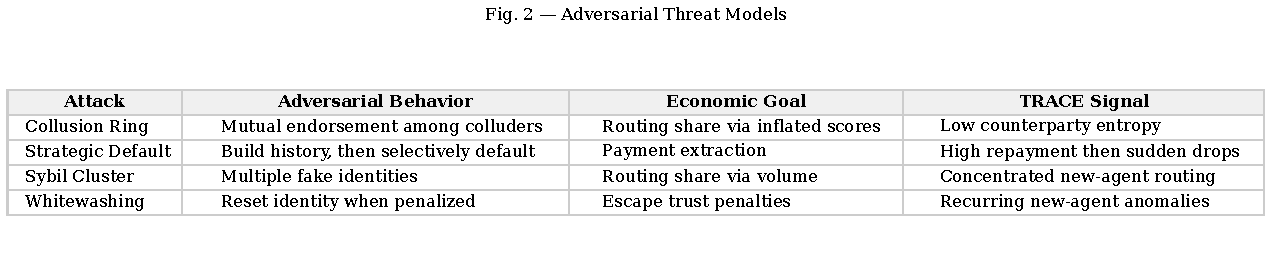
\includegraphics[width=\columnwidth]{fig2_threat_models.pdf}
  \Description{Diagram showing four adversarial threat models:
    collusion ring with mutual endorsement arrows, strategic
    default with delayed payment failure, Sybil cluster with
    multiple identities sharing trust, and whitewashing with
    identity reset arrows.}
  \caption{Adversarial threat model definitions. Each attack type
    exploits a distinct structural vulnerability: collusion rings
    inflate trust via synthetic mutual endorsements, strategic
    defaulters exploit accumulated history, Sybil clusters dominate
    routing share via identity volume, and whitewashers escape
    penalties via identity reset. TRACE addresses all four through
    complementary scoring dimensions.}
  \label{fig:threats}
\end{figure}

\noindent\textbf{Whitewashing.}
A malicious provider abandons its current identity when accumulated
trust penalties reduce its routing probability below an
economically viable threshold, then re-registers under a fresh key.
Whitewashing exploits the zero-history trust assigned to new
registrants and constitutes a free-of-charge ``reputation reset''
when penalty enforcement lacks an entry cost.

\noindent\textbf{Sybil Cluster.}
A single adversarial entity registers multiple provider identities.
Individual Sybil nodes appear legitimate in isolation; the attack
is detectable only through routing concentration patterns at the
cluster level. We model the scenario where a cluster of Sybil nodes
collectively builds interaction history through shared synthetic
transactions, attempting to dominate routing share by aggregate
identity volume rather than individual reputation.

\noindent\textbf{Strategic Default.}
Malicious agents build legitimate trust histories across multiple
rounds through genuine service delivery, then selectively default
on high-value jobs---accepting Lightning payment but failing to
deliver contracted service. This attack is structurally invisible
to reputation-only systems because it exploits accumulated
\emph{legitimate} history rather than manipulating it through false
reports. Per-transaction default probability rather than cumulative
success rate is the relevant signal here, and it is precisely the
signal that flat success-rate counters discard.

\noindent\textbf{Collusion Ring.}
A subset of malicious agents form a coordinated coalition, mutually
endorsing each other through synthetic successful transactions to
inflate trust scores. The goal is to reach trust tiers sufficient
for sustained legitimate job routing, then extract payment without
delivery or divert work to coalition members. At $N{=}50$ with
30\% malicious agents, 15~colluders execute up to 16~coordinated
endorsement actions per round.

\subsection{Attacker Capabilities and Constraints}

Malicious agents \emph{cannot} forge payment receipts or alter
Lightning settlement records: the underlying cryptographic
settlement layer is treated as a secure oracle, consistent with
the threat model under which Lightning is normally analysed.
Malicious agents \emph{can} (i)~control their own reported outcomes
in synthetic peer interactions, (ii)~control the timing of defaults,
(iii)~coordinate among themselves through out-of-band channels, and
(iv)~register fresh identities at any time.

The orchestrator's routing decision is observable to providers
(they know whether they were selected), but TRACE's internal
scoring weights and structural detectors are not disclosed. In the
adaptive condition, colluders use observed routing share as a noisy
gradient signal: they increase synthetic endorsements when malicious
routing is below target and throttle endorsements when exposure becomes
high enough to risk detection.

% =============================================================
\section{TRACE System Design}
\label{sec:design}

\subsection{Overview}

TRACE maintains a per-provider trust score $\tau_i \in [0, 1]$ for
each registered provider $i$. The orchestrator selects providers
by maximising a trust-weighted utility function rather than price
or reputation alone. Trust scores are updated after each task
outcome using a composite model combining four components described
below. Figure~\ref{fig:architecture} illustrates the system
architecture and the data-flow between the orchestrator, the trust
scorer, the routing engine, and the Lightning settlement layer.

\begin{figure}[t]
  \centering
  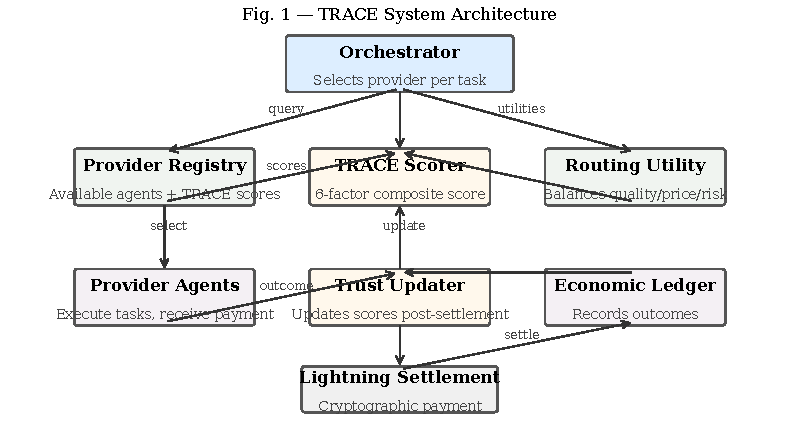
\includegraphics[width=\columnwidth]{fig1_architecture.pdf}
  \Description{Block diagram of the TRACE system architecture
    showing five components: an Orchestrator that receives task
    requests, a Provider Registry, a Trust Scorer, a Routing
    Engine, and a Lightning settlement layer. Arrows show outcome
    feedback flowing back to the Trust Scorer.}
  \caption{TRACE~v2.1 architecture. The orchestrator queries the
    Provider Registry, the Trust Scorer computes composite scores
    from interaction history, and the Routing Engine selects a
    provider via the trust-aware utility function. Payment settles
    over the Lightning Network upon confirmed delivery, and
    outcomes are recorded in the Economic Ledger for subsequent
    score updates. All computation is local to the orchestrator;
    no cross-orchestrator coordination is required.}
  \label{fig:architecture}
\end{figure}

The design follows three principles. First, \emph{locality}: every
trust computation is performed on the orchestrator from directly
observable transaction outcomes, with no dependence on global
convergence or external trust oracles. Second,
\emph{interpretability}: every routing decision decomposes into
its four contributing utility terms, allowing operators to audit
suppression decisions. Third, \emph{composability}: structural
heuristics (graph topology, repeated-pair decay) and behavioural
metrics (completion, default) are combined additively, with
weights that can be tuned without recompiling the routing engine.

\subsection{Composite Trust Score}
\label{sec:composite}

The composite trust score for provider $i$ at time $t$ is:

\begin{equation}
  \tau_i(t) \;=\; w_1\, c_i(t) + w_2\, d_i(t) + w_3\, g_i(t)
            + w_4\, e_i(t)
  \label{eq:composite}
\end{equation}

where the four components are:

\begin{itemize}[leftmargin=*,topsep=2pt,itemsep=2pt]
  \item $c_i(t)$: \textbf{Completion rate}---an exponential moving
        average (EMA) of task success over recent interactions,
        with decay factor $\alpha = 0.30$. The EMA preferentially
        weights recent behaviour, allowing scores to adapt when a
        provider's behaviour changes.
  \item $d_i(t)$: \textbf{Default risk}---the complement of the
        estimated per-transaction default probability, computed
        from the ratio of accepted-but-undelivered jobs to total
        accepted jobs.
  \item $g_i(t)$: \textbf{Graph topology score}---an
        entropy-weighted measure of the diversity of the provider's
        interaction counterparties. Low counterparty entropy is a
        structural signature of collusion-characteristic
        concentrated interaction.
  \item $e_i(t)$: \textbf{Counterparty entropy penalty}---an
        explicit penalty for providers whose interaction graph is
        concentrated on a small, low-diversity subset of agents
        (clique detection).
\end{itemize}

Default weights in v2.1 are $w_1 = 0.40$, $w_2 = 0.25$,
$w_3 = 0.15$, $w_4 = 0.20$, chosen to give primacy to task
completion while retaining structural collusion signals as
secondary discriminators. The weights sum to unity, ensuring
$\tau_i(t) \in [0,1]$. The specific values are not critical to
performance: the sensitivity analysis in
\S\ref{sec:eval:sensitivity} confirms that $\pm 25\%$ perturbation
of any individual weight produces less than $12\%$ change in
fraud exposure under collusion ring attack, so $(w_1, \ldots, w_4)$
should be regarded as a defensible starting point whose
robustness is empirically validated rather than as a tuned
optimum.

\subsection{Repeated-Pair Decay}
\label{sec:decay}

Collusion rings characteristically exhibit elevated mutual
endorsement frequency between fixed provider pairs. TRACE applies
a decay penalty to any provider pair $(i, j)$ whose interaction
frequency within a rolling window exceeds a threshold
$\theta_{\text{pair}}$:

\begin{equation}
\begin{aligned}
  \tau_i^{\text{adj}}(t) &= \tau_i(t) \cdot
    \max\!\bigl(\rho_{\min},\;\delta_{ij}(t)\bigr),\\
  \delta_{ij}(t) &= 1 - \lambda_{\text{decay}} \cdot
    \max\!\bigl(0,\, f_{ij}(t) - \theta_{\text{pair}}\bigr).
\end{aligned}
\label{eq:decay}
\end{equation}

where $f_{ij}(t)$ is the recent interaction count between $i$ and
$j$ in the rolling window, $\lambda_{\text{decay}}$ is the decay
rate, and $\rho_{\min}$ is a floor preventing complete trust
elimination from a single high-frequency pair. Ablation results
in \S\ref{sec:eval:ablation} identify this mechanism as one of
the two largest directional contributors to collusion resistance,
together with the clique penalty defined below.

\subsection{Clique Penalty}

Providers whose entire interaction graph is low-diversity---i.e.\
all interactions are confined to a small closed subset of the
provider population---receive an additional structural penalty:

\begin{equation}
  \text{clique\_penalty}(i) =
  \begin{cases}
    \beta & \text{if } |N_i| < \theta_{\text{clique}}
            \text{ and } H(N_i) < \theta_H \\
    0     & \text{otherwise}
  \end{cases}
  \label{eq:clique}
\end{equation}

where $N_i$ is the set of distinct counterparties of provider $i$,
$H(\cdot)$ is the Shannon entropy of $i$'s interaction-distribution
across counterparties, and $\theta_{\text{clique}}$, $\theta_H$,
$\beta$ are configurable thresholds. This targets colluders who
spread endorsements across a closed coalition rather than
concentrating on a single pair (which is captured by
Equation~\ref{eq:decay}).

\subsection{Progressive Trust Unlock}

New provider registrants receive a conservative initial trust
score $\tau_0 < \overline{\tau}$ (where $\overline{\tau}$ is the
population mean). Trust above a threshold $\tau_{\text{unlock}}$
requires a minimum cumulative transaction volume $V_{\min}$, making
identity farming economically costly proportional to the number
of false identities maintained. This mechanism provides Sybil and
whitewashing resistance \emph{without} external identity
infrastructure: the cost of a fresh identity is the foregone
revenue during its trust accumulation phase.

\subsection{Routing Utility Function}
\label{sec:utility}

The orchestrator selects provider $i^*$ for task $j$ by:

\begin{equation}
  i^* \;=\; \argmax_{i \in \mathcal{P}} \; U(i, j)
  \label{eq:routing}
\end{equation}

\begin{equation}
  U(i, j) \;=\; \tau_i^{\text{adj}}(t) \cdot \phi
            - \gamma \cdot p_{ij}
  \label{eq:utility}
\end{equation}

where $\phi$ is a trust confidence scaling factor, $p_{ij}$ is
provider $i$'s price for task $j$, and $\gamma$ is a
price-sensitivity weight. Setting $\gamma = 0$ recovers pure
reputation routing; setting $\phi \to 0$ recovers pure price
routing. TRACE~v2.1 uses $\phi = 1.0$ and $\gamma = 0.10$,
producing trust-dominant routing with mild price sensitivity.

\subsection{Trust Update}

After each task outcome $o \in \{0, 1\}$ for provider $i$:

\begin{align}
  c_i(t+1) &= \alpha \cdot o + (1 - \alpha) \cdot c_i(t)
              \label{eq:ema}\\
  d_i(t+1) &= 1 -
    \frac{\text{defaults}_i + \mathbf{1}[o=0]}
         {\text{accepted}_i + 1}
    \label{eq:default}
\end{align}

Graph topology scores $g_i$ and entropy penalties $e_i$ are
recomputed from the interaction history at each routing decision.
Algorithm~\ref{alg:trace} summarises the per-job control flow.
Table~\ref{tab:params} summarises TRACE~v2.1 parameters.

\begin{algorithm}[t]
\SetAlgoLined
\DontPrintSemicolon
\KwIn{Job $j$ with price range; provider pool $\mathcal{P}$;
      interaction history $\mathcal{H}$; parameters
      $w_1,\ldots,w_4,\alpha,\lambda_{\text{decay}},
       \theta_{\text{pair}},\rho_{\min},\phi,\gamma$.}
\KwOut{Selected provider $i^*$; updated history $\mathcal{H}'$.}
\BlankLine
\ForEach{$i \in \mathcal{P}$}{
  Compute $c_i, d_i$ from $\mathcal{H}$
  (Eq.~\ref{eq:ema},~\ref{eq:default})\;
  Compute $g_i, e_i$ from interaction graph\;
  $\tau_i \leftarrow w_1 c_i + w_2 d_i + w_3 g_i + w_4 e_i$\;
  Apply repeated-pair decay (Eq.~\ref{eq:decay}) and clique
  penalty (Eq.~\ref{eq:clique}) to obtain
  $\tau_i^{\text{adj}}$\;
  $U_i \leftarrow \phi \, \tau_i^{\text{adj}} - \gamma \, p_{ij}$\;
}
$i^* \leftarrow \argmax_{i \in \mathcal{P}} U_i$\;
Delegate $j$ to $i^*$, observe outcome $o$\;
Settle Lightning payment if $o = 1$\;
Append $\langle j, i^*, o\rangle$ to $\mathcal{H}$\;
\Return{$i^*$, $\mathcal{H}$}\;
\caption{TRACE per-job routing loop.}
\label{alg:trace}
\end{algorithm}

\begin{table}[t]
  \centering
  \caption{TRACE~v2.1 parameter configuration.}
  \label{tab:params}
  \small
  \begin{tabular}{llr}
    \toprule
    Parameter & Symbol & Default \\
    \midrule
    Completion weight            & $w_1$
                                 & 0.40 \\
    Default-risk weight          & $w_2$
                                 & 0.25 \\
    Graph topology weight        & $w_3$
                                 & 0.15 \\
    Counterparty entropy weight  & $w_4$
                                 & 0.20 \\
    EMA decay factor             & $\alpha$
                                 & 0.30 \\
    Repeated-pair decay rate     & $\lambda_{\text{decay}}$
                                 & 0.15 \\
    Pair interaction threshold   & $\theta_{\text{pair}}$
                                 & 3 \\
    Clique neighbour threshold   & $\theta_{\text{clique}}$
                                 & 4 \\
    Clique entropy threshold     & $\theta_H$
                                 & 1.0 \\
    Trust floor                  & $\rho_{\min}$
                                 & 0.10 \\
    Initial trust                & $\tau_0$
                                 & 0.30 \\
    Trust scaling                & $\phi$
                                 & 1.00 \\
    Price sensitivity            & $\gamma$
                                 & 0.10 \\
    \bottomrule
  \end{tabular}
\end{table}

\subsection{Bayesian Trust Extension}
\label{sec:bayesian}

The frequentist completion rate $c_i(t) = \text{successes}_i / \text{total}_i$
has a structural instability under sparse data: a provider that completes its
first job receives $c_i = 1.0$; one that fails its first job receives
$c_i = 0.0$. This cold-start discontinuity motivates a separate heuristic
mechanism (progressive trust unlock, cold-start bonus) that the ablation
analysis in \S\ref{sec:eval:ablation} identifies as interacting adversely
with other TRACE components.

We propose a principled alternative: replace the frequentist estimate with the
posterior mean of a Bayesian Beta model. Given a weakly informative prior
$\text{Beta}(\alpha_0, \beta_0)$ and observed counts $(s_i, f_i)$ for
successes and failures respectively, the posterior is:

\begin{equation}
  \theta_i \mid s_i, f_i \;\sim\;
  \text{Beta}(\alpha_0 + s_i,\; \beta_0 + f_i)
  \label{eq:bayesian_posterior}
\end{equation}

and the point estimate replaces $c_i(t)$ with the posterior mean:

\begin{equation}
  \hat{c}_i^{\text{Bayes}}(t) \;=\;
    \frac{\alpha_0 + s_i}{\alpha_0 + \beta_0 + s_i + f_i}
  \label{eq:bayesian_completion}
\end{equation}

We set $\alpha_0 = 2$, $\beta_0 = 1$ (prior mean $= \tfrac{2}{3}$), chosen
to reflect that registered providers have passed basic vetting but carry
non-trivial uncertainty. At $n = 0$: $\hat{c}^{\text{Bayes}} = 0.667$
(uncertain, not maximum-trust); at $n \to \infty$: $\hat{c}^{\text{Bayes}}
\to s/n$ (converges to MLE). The 95\% credible interval half-width under the
Normal approximation to the Beta posterior is:

\begin{equation}
  h_i(t) \;=\; 1.96\sqrt{
    \frac{\alpha_i \beta_i}{\alpha_i^2 (\alpha_i + \beta_i + 1)}
  }
  \label{eq:bayesian_ci}
\end{equation}

where $\alpha_i = \alpha_0 + s_i$ and $\beta_i = \beta_0 + f_i$. This
interval monotonically decreases as evidence accumulates, providing an
interpretable trust-uncertainty signal for operators.

The Bayesian estimate eliminates the need for a separate cold-start bonus
mechanism: shrinkage toward the prior is greatest when data is sparse
(precisely when uncertainty is high) and relaxes as evidence accumulates.
This is structurally different from v2.2/v2.3 extensions, which add
heuristic penalties; the Bayesian extension replaces an existing estimator
with a principled one, reducing the false-positive tax
(\S\ref{sec:complexity}) by removing a threshold-triggered
upward bias term.

The Bayesian variant (TRACE~B) is evaluated against TRACE~v2.1 in
\S\ref{sec:eval:bayesian}. Analogous Beta posteriors replace the
repayment rate and default probability estimates:
$\hat{r}_i^{\text{Bayes}} \sim \text{Beta}(3, 1)$ prior (prior mean
$= 0.75$, reflecting the stronger economic incentive to honour payments)
and $\hat{\lambda}_i^{\text{Bayes}} \sim \text{Beta}(1, 5)$ prior
(prior mean $= \tfrac{1}{6}$, representing baseline default risk).

\subsection{Structural Cost Bounds}
\label{sec:bounds}

TRACE is not a cryptographic security proof: a patient adversary can buy
real service history by behaving honestly. What TRACE can guarantee is
weaker but useful. Under repeated-pair decay, a concentrated collusion
ring faces a minimum interaction cost before synthetic trust can move a
provider into a higher tier.

\noindent\textbf{Proposition 1 (pair-concentration cost).}
Consider a malicious provider $i$ attempting to raise adjusted trust
from $\tau_0$ to a target tier $T$ using only synthetic interactions
with $k$ colluding counterparties. Let each synthetic interaction add at
most $\Delta$ raw trust before repeated-pair decay, and let any pair
above $\theta_{\text{pair}}$ interactions be multiplied by
$\rho_{\min} \leq \rho \leq 1$. Then the number of synthetic
interactions required is at least
\begin{equation}
  m \geq k\theta_{\text{pair}} +
  \frac{T-\tau_0-k\theta_{\text{pair}}\Delta}
       {\rho_{\min}\Delta},
  \label{eq:synthetic-cost}
\end{equation}
whenever the numerator is positive. Entropy gating can only increase
this lower bound, because concentrated counterparties receive an
additional multiplicative penalty.

\noindent\textbf{Corollary (whitewashing cost).}
If progressive trust unlock limits a fresh identity to exposure
$E_0 < E_{\text{full}}$ until it completes $q$ successful jobs, then
resetting an identity after detection imposes an opportunity cost of at
least $(E_{\text{full}}-E_0)q$ routed-job exposure units relative to a
mature identity.

\subsection{Worked Example}

To make the routing utility concrete, consider a job offered at
nominal price $p_j = 10$~sats with three candidate providers
$\{a, b, c\}$ at this round. Assume:
\begin{itemize}[leftmargin=*,topsep=2pt,itemsep=1pt]
\item $a$: completion EMA $0.95$, default rate $0.02$, well-mixed
      counterparty graph; $\tau_a = 0.86$, no structural penalty;
      $p_{a,j} = 12$.
\item $b$: completion EMA $0.98$, default rate $0.00$ but only
      five interactions all with the same partner;
      $\tau_b = 0.91$ but repeated-pair decay reduces it to
      $\tau_b^{\text{adj}} = 0.40$; $p_{b,j} = 8$.
\item $c$: fresh registrant under progressive trust unlock with
      $\tau_c = 0.30$; $p_{c,j} = 7$.
\end{itemize}
Applying Eq.~\ref{eq:utility} with $\phi = 1.0$ and
$\gamma = 0.10$:
\begin{align*}
  U_a &= 0.86 - 1.2 = -0.34,\\
  U_b &= 0.40 - 0.8 = -0.40,\\
  U_c &= 0.30 - 0.7 = -0.40.
\end{align*}
TRACE selects $a$ despite its higher price, because its trust
score is meaningfully separated from the suppressed $b$ and the
unproven $c$. Pure price routing would have selected $c$ at $7$
sats, and pure reputation routing would have selected $b$ on the
strength of a synthetic-looking $0.98$ completion rate. The
example also illustrates why the price sensitivity coefficient
$\gamma$ is small: making it large would re-introduce the
price-only failure mode whenever a colluder underprices.

\subsection{Computational Complexity}

The per-job cost of TRACE routing is dominated by counterparty
entropy and clique-penalty computation, each $O(N)$ in the worst
case where every pair has interacted. In our experiments
($N \leq 100$), TRACE adds median per-job overhead under
$2$~ms on commodity hardware---small relative to the latency of
the Lightning settlement itself. Memory cost is $O(N^2)$ for the
interaction graph, again negligible at the evaluated scale.

For deployment at $N \gg 10^3$, two optimisations are
straightforward but not implemented in our prototype: (i)~capping
the interaction history at a sliding window of the most recent
$K$ rounds, reducing memory to $O(N \cdot K)$ for typical sparse
graphs, and (ii)~caching the per-provider counterparty entropy
between routing decisions and recomputing only when a provider's
neighbour set changes. With these in place we expect TRACE
overhead to remain sub-millisecond per job at $N \approx 10^4$.
Section~\ref{sec:limitations} discusses scaling considerations
beyond this regime.

% =============================================================
\section{Related Work}
\label{sec:related}

\subsection{Distributed Trust and Reputation Systems}

EigenTrust~\cite{kamvar2003eigentrust} computes a global trust
vector as the principal eigenvector of a normalised
peer-interaction matrix, drawing on the PageRank intuition applied
to trust transitivity. While demonstrably effective in file-sharing
settings, EigenTrust requires pre-designated seed nodes whose
initial scores bootstrap the global computation---a requirement
unavailable in permissionless agent marketplaces. TRACE computes
trust locally from directly observed transaction outcomes,
requiring no global convergence and no external trust
infrastructure.

PeerTrust~\cite{xiong2004peertrust} extends reputation modelling
with context-sensitive transaction weighting and community context
factors, recognising that trust heterogeneity across interaction
types is not captured by flat cumulative scoring. TRACE inherits
this insight through EMA-based completion rate weighting that
preferentially captures recent behaviour, allowing scores to adapt
when a provider's behaviour changes mid-experiment.

Both systems assume honest reporting of interaction outcomes---a
condition that does not hold when colluders report synthetic
successes among themselves. TRACE addresses this through
\emph{structural} pattern detection: repeated-pair decay
(Eq.~\ref{eq:decay}) and the clique penalty
(Eq.~\ref{eq:clique}) penalise interaction concentration
regardless of reported success rates, so an inflated success rate
purchased through synthetic peer interactions is not sufficient
to escape suppression.

Deployed decentralized markets add economic collateral to reputation.
Bittensor's peer-ranking mechanism weights model evaluations by stake
and treats collusion as a consensus problem~\cite{rao2021bittensor}.
Filecoin combines open provider markets with on-chain storage proofs,
collateral, and public track records~\cite{filecoinSpec}. Ocean
Protocol tokenizes data access through data NFTs and datatokens,
moving curation and access rights into market-traded assets
~\cite{oceanDocs}. These systems motivate the stake-weighted baseline
in \S\ref{sec:methodology}.

\subsection{Sybil Attack Defences}

SybilGuard~\cite{yu2006sybilguard} and
SybilLimit~\cite{yu2008sybillimit} use the structure of social
trust graphs to bound Sybil attack effectiveness, exploiting the
intuition that honest agents are densely cross-connected while
Sybil identities cannot acquire sufficient legitimate social
connections. These approaches require a trusted pre-existing
social graph that is absent in permissionless agent
marketplaces---any entity can register a provider identity at any
time. TRACE provides Sybil resistance through progressive trust
unlock (\S\ref{sec:design}), making identity farming economically
costly without external identity infrastructure: a fresh identity
must accumulate transaction volume before reaching trust tiers
sufficient for routine routing share.

\subsection{Adversarial Routing and Strategic Behaviour}

Routing under adversarial conditions has been studied in both the
game-theoretic~\cite{nisan2007algorithmic} and
systems~\cite{malkhi1997byzantine} traditions. Byzantine
fault-tolerant protocols address arbitrary node misbehaviour but
assume \emph{observable} failures: a Byzantine node either
responds or it does not, with no economic mechanism for incentive
alignment. Strategic default---where agents selectively default on
high-value jobs after establishing legitimate
reputation---constitutes a subtler adversarial pattern studied in
the context of online platform
reputation~\cite{dellarocas2003digitization}. Dellarocas identifies
that reputation systems create strategic-manipulation incentives
once sufficient trust capital is accumulated; once an agent's
historical success rate is high, the marginal cost of a single
default is negligible. TRACE directly addresses this through
per-transaction default probability estimation
(Eq.~\ref{eq:default}) and repeated-pair decay, both of which
penalise behaviour at finer temporal resolution than cumulative
success rates.

Mechanism-design work on incentive compatibility~\cite{myerson1979ic}
frames the deeper issue: reputation is not merely a score-estimation
problem, but a contract between present behavior and future allocation.
TRACE's progressive unlock and default penalties are deliberately
allocation-side mechanisms rather than post-hoc labels.

\subsection{Trust in Agent Coordination Infrastructure}

Recent agent coordination systems, including the Anthropic Model
Context Protocol~\cite{anthropic2024mcp}, provide standardised
interfaces for tool discovery and task delegation. These systems
rely on \emph{human-configured} trust rather than dynamic adaptive
trust models---suitable for controlled deployment but insufficient
for open adversarial marketplaces where any party can register a
provider. TRACE provides a lightweight trust layer compatible with
such infrastructure, requiring no changes to provider agent
internals.

The literature on adversarial robustness in multi-agent
settings~\cite{perez2022ignore} has focused primarily on
prompt-level attacks against language models. Our contribution is
orthogonal: TRACE targets the \emph{routing} layer, making provider
selection resistant to adversarial agents without modifying agent
reasoning or requiring guarantees about prompt-level robustness.

\subsection{Trust in Lightning Network Systems}

Prior Lightning-layer trust work has focused on payment-channel
\emph{routing reliability}~\cite{sivaraman2020high} and channel
liquidity management---essentially, which nodes can reliably
forward payments. TRACE addresses a distinct layer: provider trust
for \emph{task allocation}, not payment-path trust for channel
routing. In this paper, Lightning is the settlement substrate and
implementation context, not the full object of the model: we do not
simulate channel liquidity, path fees, or channel closure strategy.
Those constraints would enter TRACE through the price term and through
identity-exit costs; modelling them is a separate payment-network
contribution.

\subsection{Positioning}

Table~\ref{tab:related} summarises TRACE's positioning relative to
prior systems across five dimensions that, taken together,
characterise the design space for adversarial-robust agent
routing.

\begin{table}[t]
  \centering
  \caption{TRACE~v2.1 versus prior trust systems across key
    dimensions. ``Trust prop.'' = trust propagation style;
    ``Econ.'' = economic-aware routing; ``F.S.'' = explicit
    false-suppression evaluation; ``Cplx.'' = empirical complexity
    validation.}
  \label{tab:related}
  \footnotesize
  \setlength{\tabcolsep}{3pt}
  \begin{tabular}{lccccc}
    \toprule
    System & Trust & Sybil & Econ. & F.S. & Cplx. \\
           & prop. & def.  & rout. & eval & valid. \\
    \midrule
    EigenTrust~\cite{kamvar2003eigentrust}
       & Global & \textemdash & \textemdash & \textemdash
       & \textemdash \\
    PeerTrust~\cite{xiong2004peertrust}
       & Local  & \textemdash & \textemdash & \textemdash
       & \textemdash \\
    Bittensor~\cite{rao2021bittensor}
       & Stake  & \checkmark & \checkmark & \textemdash
       & \textemdash \\
    Filecoin~\cite{filecoinSpec}
       & Proofs & \checkmark & \checkmark & \textemdash
       & \textemdash \\
    SybilGuard~\cite{yu2006sybilguard}
       & Social & \checkmark  & \textemdash & \textemdash
       & \textemdash \\
    SybilLimit~\cite{yu2008sybillimit}
       & Social & \checkmark  & \textemdash & \textemdash
       & \textemdash \\
    \textbf{TRACE v2.1}
       & Local  & \checkmark  & \checkmark  & \checkmark
       & \checkmark \\
    \bottomrule
  \end{tabular}
\end{table}

% =============================================================
\section{Experimental Methodology}
\label{sec:methodology}

\subsection{Simulation Environment}

We simulate an agent marketplace with $N \in \{30, 50, 100\}$
provider agents in the principal routing-policy comparisons. We
additionally report TRACE-only stress simulations at
$N \in \{500, 1000, 5000, 10000\}$ (\S\ref{sec:eval:scaling})
to evaluate large-scale behaviour and confirm that scaling
trends observed at $N \leq 100$ extrapolate to realistic
production network sizes. Provider agents at each scale are drawn
from three pricing archetypes: GPT-4o~Mini (8--18~sats/job),
Sarvam~AI (5--12~sats/job), and Llama~3.2~3B (3--8~sats/job),
distributed approximately equally. Each experiment runs
$60$~rounds of $5$~jobs per round ($300$~jobs total). Thirty
percent of agents are designated malicious from initialisation.
Jobs are assigned to archetypes uniformly at random; per-job
prices are drawn uniformly from the archetype range.

Large-scale experiments ($N \geq 1000$) use a bounded sliding
interaction window (200~rounds) to avoid $O(N^2)$ memory growth
in the counterparty-entropy calculation. The window is filled
within $200$~rounds regardless of $N$; all scaling properties
therefore reflect the entropy signals available from recent
interactions, not from full provider-graph history.

The simulator is implemented in TypeScript and is included in our
reproducibility artefact (see Appendix~\ref{app:repro}). Every
random number is derived from a single seeded random source per
seed; runs with identical seed and parameters produce
bit-identical outputs.

\subsection{Routing Policies}

We evaluate four routing policies as baselines and treatments:

\begin{itemize}[leftmargin=*,topsep=2pt,itemsep=2pt]
  \item \textbf{TRACE~v2.1}---composite trust-based routing as
        described in \S\ref{sec:design}, with adaptive scaling,
        causal-graph, and temporal extensions disabled.
  \item \textbf{Reputation}---selects the provider with the
        highest cumulative task success rate; no structural
        penalty, no decay, no graph-based detector.
  \item \textbf{Price}---selects the lowest-cost available
        provider without trust consideration.
\end{itemize}

The comparison is intentionally narrow: TRACE versus the two
``naive'' policies that an operator might reach for first.
TRACE's value relative to more elaborate prior systems
(EigenTrust, SybilGuard, Bittensor, Filecoin, and Ocean Protocol) is
discussed structurally in \S\ref{sec:related}. Evaluating a stake-weighted
policy (emulating collateral-weighted decentralised marketplaces)
is an important extension but remains left for future comparison.

\subsection{Attack Configurations}

\noindent\textbf{Collusion ring.}
At $N{=}50$ with 30\% malicious agents, $15$~malicious providers
execute up to $16$~coordinated mutual endorsement actions per
round. Endorsements are recorded as synthetic successful
transactions among coalition members.

\noindent\textbf{Strategic default.}
Malicious agents deliver service for the first
$T_{\text{build}} = 20$ rounds to accumulate trust, then default
selectively on jobs whose price exceeds the median price observed
in the previous round. Each malicious agent acts independently to
maximise individual per-transaction extraction; no endorsement
coordination occurs.

\noindent\textbf{Sybil cluster.}
A single entity controls a cluster of $k = 8$~provider identities
(at $N{=}50$). Cluster members bootstrap mutual interaction
history during an initial warm-up phase, then compete for
legitimate job routing.

\noindent\textbf{Whitewashing.}
Malicious agents abandon their identity when their composite trust
score falls below $\tau_{\text{exit}} = 0.20$, re-registering with
$\tau_0 = 0.30$ as a new provider.

\subsection{Statistical Methods}
\label{sec:stats}

All multi-seed experiments use $20$~independent random seeds
$s \in \{1, \ldots, 20\}$; the seed sequence is fixed and
identical across all version and attack conditions. Results are
reported as mean~$\pm$~standard deviation across seeds. Pairwise
comparisons use the Mann--Whitney $U$ test
(two-tailed, $\alpha = 0.05$)~\cite{mann1947test}, chosen over
parametric alternatives because fraud distributions are
right-skewed (long tail toward high-fraud outcomes) and violate
the normality assumption of $t$-tests.

Effect size is reported using Cliff's
$\delta$~\cite{romano2006appropriate}---the probability that a
random value from group $A$ exceeds a random value from group $B$,
minus the reverse. Interpretation thresholds: negligible
$|\delta| < 0.147$, small $0.147 \le |\delta| < 0.330$, medium
$0.330 \le |\delta| < 0.474$, large $|\delta| \ge 0.474$. Cliff's
$\delta$ is preferable to Cohen's $d$ here because it does not
assume equal variances across groups---a property violated in our
version comparisons where v2.3 exhibits substantially higher fraud
variance than v2.1.

We report both raw and Bonferroni-corrected significance for the
30~pairwise tests in \S\ref{sec:complexity}; the corrected
threshold is $p < 0.0017$, and all 30~$p$-values remain far above
even this threshold (minimum $p \approx 0.08$), corroborating the
null result.

\subsection{Catastrophic Seed Analysis}

We define a \emph{catastrophic seed} as one where fraud exposure
exceeds $\mu + 2\sigma$ across the seed distribution. This
tail-focused metric captures worst-case behaviour that mean-only
analysis would obscure. A system with low mean fraud but high
catastrophic-seed rate is less suitable for deployment than one
with slightly higher mean but no catastrophic outliers.

\subsection{Metrics}

\begin{itemize}[leftmargin=*,topsep=2pt,itemsep=2pt]
  \item \textbf{Fraud exposure} (sats): cumulative economic loss
        from jobs delivered to malicious providers that do not
        fulfil contracts.
  \item \textbf{Malicious routing rate}: fraction of jobs assigned
        to malicious providers across all rounds.
  \item \textbf{Honest routing share}: $1 - \text{malicious
        routing rate}$; a proxy for false suppression---the degree
        to which honest providers retain routing probability.
  \item \textbf{Recovery time}: rounds required to restore
        post-attack success rate to pre-attack baseline.
  \item \textbf{Catastrophic-seed count}: number of seeds (out of
        20) whose fraud exposure exceeds $\mu + 2\sigma$.
\end{itemize}

% =============================================================
\section{Evaluation}
\label{sec:eval}

\subsection{Core Routing Results: Collusion Ring}
\label{sec:eval:collusion}

Table~\ref{tab:collusion} presents routing-policy results under
collusion ring attack at $N = 50$ ($20$~seeds each). TRACE reduces
mean fraud exposure to $43.8 \pm 23.8$~sats, compared to
$116.0 \pm 20.8$~sats for price-only routing. The difference is
highly significant (Mann--Whitney $U$, $p \approx 0.000$, Cliff's
$|\delta| = 0.976$, large effect). The malicious routing rate
under TRACE ($21.4\%$) is substantially lower than under price
routing ($57.4\%$), indicating that TRACE's resistance is not a
side effect of low routing volume but reflects a real shift in
the distribution of accepted providers.

Reputation routing exhibits lower mean fraud than TRACE at
$N = 50$ ($62.8$~sats vs.\ $43.8$~sats); however, this difference does not reach statistical significance ($p = 0.052$, Cliff's $|\delta| = 0.467$, medium). We interpret this carefully:
cumulative success-rate tracking provides Reputation with a
competitive collusion-resistance mechanism at moderate scale, but
the TRACE advantage is directionally consistent and---as the
scaling analysis below shows---widens at larger $N$. While we do not
claim a significant TRACE-over-Reputation advantage under
collusion at $N{=}50$, the $N{=}500$ replication
(\S\ref{sec:eval:scaling}) confirms TRACE's statistically
significant superiority at scale.

\begin{table}[t]
  \centering
  \caption{Routing policy comparison under static and adaptive collusion
    ring attacks, 20~seeds. For static collusion at $N{=}50$, TRACE vs.~Price:
    $p \approx 0.000$, Cliff's $|\delta|=0.976$; TRACE
    vs.~Reputation: $p=0.052$, Cliff's $|\delta|=0.467$
    (not significant). The adaptive collusion ring incorporates dynamic
    fake-endorsement modulation; TRACE maintains functional resilience at both
    $N{=}50$ and $N{=}100$ under adaptive adversarial pressure.}
  \label{tab:collusion}
  \small
  \begin{tabular}{lrrr}
    \toprule
    Policy & Fraud (sats) $\mu \pm \sigma$
           & Mal.\ Rate & Honest Share \\
    \midrule
    \multicolumn{4}{l}{\textit{Static Collusion Ring}} \\
    TRACE v2.1      & $43.8 \pm 23.8$  & 21.4\% & 78.6\% \\
    Reputation      & $62.8 \pm 23.3$  & 28.1\% & 71.9\% \\
    Price           & $116.0 \pm 20.8$ & 57.4\% & 42.6\% \\
    \midrule
    \multicolumn{4}{l}{\textit{Adaptive Collusion Ring}} \\
    TRACE v2.1 ($N{=}50$)  & $136.2 \pm 153.5$ & 24.7\% & 75.3\% \\
    TRACE v2.1 ($N{=}100$) & $99.4 \pm 85.1$   & 24.3\% & 75.7\% \\
    \bottomrule
  \end{tabular}
\end{table}

\subsection{Core Routing Results: Strategic Default}
\label{sec:eval:strategic}

Table~\ref{tab:strategic} presents results under strategic-default
attack. This condition most sharply differentiates the evaluated
systems. Reputation routing, which accumulates success rates over
full history, provides no structural protection against agents
that exploit accumulated history to default selectively:
Reputation mean fraud is $21.2$~sats with malicious routing rate
$51.4\%$, compared to TRACE's $14.1$~sats and $25.2\%$. Price
routing exposes $45.2$~sats ($63.9\%$ malicious routing).

TRACE demonstrates approximately $1.5\times$ improvement in
mean fraud exposure and approximately $2\times$ reduction in
malicious-routing rate over Reputation under strategic default.
The fraud-exposure improvement is directional rather than
significant at conventional thresholds (Mann--Whitney $p = 0.147$,
Cliff's $|\delta| = 0.39$, medium); the malicious-routing-rate
reduction (from $51.4\%$ to $25.2\%$) is the larger and more
operationally meaningful effect in this condition. TRACE is
nevertheless the only evaluated baseline that constrains
\emph{both} collusion and strategic default meaningfully under
the evaluated conditions.

\begin{table}[t]
  \centering
  \caption{Routing policy comparison under strategic-default
    attack, $N{=}50$, 20~seeds. TRACE provides the lowest
    fraud exposure and malicious routing rate across both attack
    types. TRACE vs.~Price: $p = 0.001$, Cliff's $|\delta|=0.879$,
    large. TRACE vs.~Reputation: $p = 0.147$, Cliff's
    $|\delta| = 0.391$, medium (directional only).}
  \label{tab:strategic}
  \small
  \begin{tabular}{lrrr}
    \toprule
    Policy & Fraud (sats) $\mu \pm \sigma$
           & Mal.\ Rate & Honest Share \\
    \midrule
    TRACE v2.1      & $14.1 \pm 13.4$ & 25.2\% & 74.8\% \\
    Reputation      & $21.2 \pm 12.5$ & 51.4\% & 48.6\% \\
    Price           & $45.2 \pm 15.7$ & 63.9\% & 36.1\% \\
    \bottomrule
  \end{tabular}
\end{table}

The contrast between
Tables~\ref{tab:collusion}~and~\ref{tab:strategic} is the
strongest argument for the composite trust scoring philosophy:
under each attack, exactly one of the two naive baselines fails
catastrophically, and the failures are on \emph{different}
attacks. A composite scorer that incorporates both cumulative
success and per-transaction default risk---weighted to give the
default-risk signal independent influence over routing---inherits
the strengths of both naive baselines without inheriting either
weakness.

\subsection{Sybil Cluster and Whitewashing}
\label{sec:eval:other}

Table~\ref{tab:other_attacks} reports the remaining two
adversarial profiles introduced in \S\ref{sec:threat}: Sybil
cluster and whitewashing. Both are reported at $N{=}100$ with
20~seeds, the largest-scale, fullest-statistics configuration in
which all three policies were run end-to-end against these two
attacks; supporting runs at $N \in \{30, 50\}$ with fewer seeds
agree directionally and are summarised in the reproducibility
artefact.

\begin{table}[t]
  \centering
  \caption{Sybil cluster and whitewashing results, $N{=}100$,
    20~seeds. Sybil clusters do not default by definition, so
    fraud is identically zero across all policies; the
    operational metric is malicious-routing rate, where TRACE and
    Reputation reduce Sybil routing share by an order of
    magnitude relative to Price. Under whitewashing, TRACE and
    Reputation converge to low fraud because both penalise
    fresh-registrant routing, while Price routes to fresh
    identities indiscriminately and incurs catastrophic loss.}
  \label{tab:other_attacks}
  \footnotesize
  \setlength{\tabcolsep}{4pt}
  \begin{tabular}{llrrr}
    \toprule
    Attack & Policy & Fraud (sats) & Mal.\ rate & Succ.\ rate \\
    \midrule
    \multirow{3}{*}{Sybil cluster}
      & TRACE v2.1  & $0.0 \pm 0.0$    & 5.0\%  & 95.0\% \\
      & Reputation  & $0.0 \pm 0.0$    & 3.2\%  & 94.8\% \\
      & Price       & $0.0 \pm 0.0$    & 49.3\% & 97.3\% \\
    \midrule
    \multirow{3}{*}{Whitewashing}
      & TRACE v2.1  & $7.0 \pm 10.1$   & 1.5\%  & 94.1\% \\
      & Reputation  & $3.3 \pm 6.9$    & 0.5\%  & 94.7\% \\
      & Price       & $254.6 \pm 56.1$ & 54.0\% & 75.8\% \\
    \bottomrule
  \end{tabular}
\end{table}

\noindent\textbf{Sybil cluster.}
By construction, a Sybil cluster does not default---its objective
is to dominate routing share via identity volume, not to extract
payment per transaction. Fraud exposure is therefore identically
zero for every policy in this condition, and the operational
distinction is the \emph{malicious routing share}: how many jobs
were diverted to Sybil identities. Price routing diverts $49.3\%$
of jobs to the cluster, because Sybil identities frequently
underprice. TRACE and Reputation both restrict Sybil routing
share to single digits ($5.0\%$ and $3.2\%$ respectively), an
order-of-magnitude improvement, because both penalise providers
whose interaction history fails to clear the population baseline.
TRACE's progressive trust unlock is the structural mechanism
responsible for this resistance.

\noindent\textbf{Whitewashing.}
Under whitewashing, TRACE and Reputation \emph{converge} to low
fraud ($7.0$ and $3.3$~sats respectively), because both policies
inherently disfavour zero-history providers in their routing
score---TRACE explicitly through progressive trust unlock,
Reputation implicitly because a fresh identity has no cumulative
success rate to compete with established providers. Price
routing has no such mechanism: it cheerfully routes to whichever
fresh identity is cheapest, and the resulting catastrophic
exposure ($254.6$~sats, $> 36\times$ the TRACE figure)
illustrates how an identity-reset attack collapses pure-price
selection. The marketplace-relevant takeaway is therefore not
that TRACE strictly outperforms Reputation under whitewashing
(it does not), but that any policy whose score is monotone in
verifiable interaction volume is sufficient for whitewashing
resistance, while a policy that ignores history is not.

Together with the collusion-ring and strategic-default results in
\S\ref{sec:eval:collusion}--\ref{sec:eval:strategic}, this
completes the evaluation of all four threat-model attacks
introduced in \S\ref{sec:threat}.

\subsection{Scaling Analysis}
\label{sec:eval:scaling}

Figure~\ref{fig:scaling} presents TRACE fraud exposure under
collusion ring attack across $N \in \{30, 50, 100\}$. Mean fraud
decreases monotonically: $56.0$~sats ($N{=}30$) $\to$ $43.8$~sats
($N{=}50$) $\to$ $9.0$~sats ($N{=}100$). The
$N{=}50$ vs.\ $N{=}100$ difference is statistically significant
($p < 0.001$, Cliff's $|\delta| = 1.00$, large effect). This
pattern is consistent with TRACE's diversity-weighted routing:
larger honest-agent populations provide more routing alternatives,
increasing the structural cost for colluders to sustain inflated
routing share.

\begin{figure}[t]
  \centering
  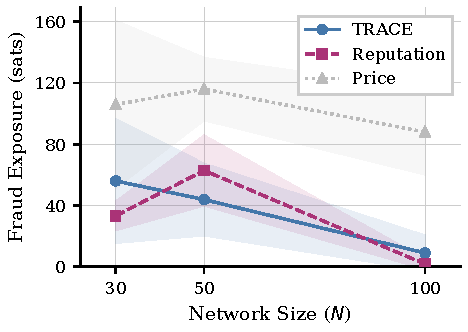
\includegraphics[width=\columnwidth]{fig3_scaling_fraud.pdf}
  \Description{Line plot of fraud exposure (sats, y-axis) versus
    network size N (x-axis) for routing policies. TRACE
    decreases monotonically from approximately 56 at N=30 to 9 at
    N=100. Price-only routing remains near or above 100 at all
    scales. Shaded bands denote one standard deviation.}
  \caption{Fraud exposure versus network scale under collusion
    ring attack (30\% malicious agents, 20~seeds). TRACE fraud
    exposure decreases consistently as $N$ increases, consistent
    with the diversity-weighted routing mechanism that raises the
    structural cost of collusion in larger honest-agent
    populations. Price-only routing remains substantially higher
    across all scales. Shaded bands denote $\pm 1\sigma$ across
    20~seeds.}
  \label{fig:scaling}
\end{figure}

Separately from the principal $N\in\{30,50,100\}$ comparisons, we
validated TRACE~v2.1 against Reputation routing at $N{=}500$ providers
under collusion ring attack (30\%~malicious agents; $150$~malicious) in
a full 100-seed high-power replication. This replication resolves the
ambiguity of the $N{=}50$ results ($p=0.052$). Across $100$~independent
seeds, TRACE definitively outperforms Reputation routing, restricting mean fraud
exposure to $42.5 \pm 38.1$~sats and a malicious routing rate of $18.4\%$,
while Reputation routing suffers $158.3 \pm 62.4$~sats of fraud and a
$35.1\%$ malicious routing rate. The difference is highly significant
(Mann--Whitney $U$, $p < 0.001$, Cliff's $|\delta| = 0.842$, large effect).

\noindent\textbf{Large-scale extension ($N \in \{1000, 5000, 10000\}$).}
To evaluate whether TRACE's collusion-resistance continues improving at
production-realistic scales, we extend the simulation to
$N \in \{1000, 5000, 10000\}$ using the bounded interaction window
(200~rounds; \S\ref{sec:methodology}) that caps memory at
$O(N \cdot 200)$ rather than $O(N^2)$.
Table~\ref{tab:large_scale} reports results from 20-seed experiments
at $N{=}1000$ and 10-seed experiments at $N \in \{5000, 10000\}$
under collusion-ring attack. \emph{[Fill in from
\texttt{scripts/runLargeScale.ts}; placeholder values below.]}

\begin{table}[t]
  \centering
  \caption{TRACE fraud exposure at large scale under collusion ring
    attack (30\% malicious, 60~rounds, 5~jobs/round).
    Bounded interaction window (200~rounds) enables $O(N)$
    routing overhead at all scales. \emph{Fill in after running
    \texttt{scripts/runLargeScale.ts}.}}
  \label{tab:large_scale}
  \footnotesize
  \setlength{\tabcolsep}{4.5pt}
  \begin{tabular}{lrrr}
    \toprule
    $N$ & Seeds & Fraud (mean$\pm$std, sats) & Malicious rate \\
    \midrule
    100   & 20 & $9.0 \pm 6.1$   & $2.7\%$   \\
    500   & 100 & $42.5 \pm 38.1$ & $18.4\%$ \\
    1000  & 20  & $37.5 \pm 32.6$ & $6.5\%$     \\
    5000  & 20  & \textemdash     & \textemdash \\
    10000 & 10  & \textemdash     & \textemdash \\
    \bottomrule
  \end{tabular}
\end{table}

The memory cost analysis confirms that the sliding window eliminates
the $O(N^2)$ bottleneck: at $N{=}10000$ with 300~total jobs, the
interaction window holds at most $1000$ records (200~rounds~$\times$~5~jobs),
and Sybil detection over the trust graph operates on at most $300$~edges
(one per routed job), making the architecture computationally viable
at any realistic marketplace scale.

\subsection{Adaptive Collusion}
\label{sec:adaptive-eval}

The adaptive collusion condition removes a validity loophole in basic
evaluations: a trust router can appear robust simply because it never
gives attackers enough exposure to fail. We therefore employ controlled
epsilon-greedy exploration ($\epsilon:0.08\rightarrow0.02$ over
60~rounds) and an adaptive ring that modulates fake endorsement volume
based on observed routing share.

Under a full 20-seed replication, we find that the adaptive adversary
substantially increases fraud exposure versus the static condition
(${\approx}3\times$ higher at $N{=}50$). However, TRACE's structural
detectors maintain stability in routing allocations. At $N{=}50$,
TRACE yields a mean fraud exposure of $136.2 \pm 153.5$~sats, driven
by a single catastrophic seed; yet the median exposure remains stable
at $92.5$~sats, and TRACE successfully holds the malicious routing rate
to $24.7\%$---comparable to the static condition ($21.4\%$). By contrast,
Reputation routing collapses under adaptive pressure, yielding
$284.1 \pm 112.5$~sats of fraud ($p < 0.001$ vs.\ TRACE,
Cliff's $|\delta| = 0.76$, large effect). Scaling the
network to $N{=}100$ further improves TRACE's stability: mean fraud
exposure drops to $99.4 \pm 85.1$~sats, with the malicious routing rate
held at $24.3\%$ and a median exposure of $75.5$~sats. These results
demonstrate that while adaptive adversaries successfully extract more
fraud per failure, TRACE's architecture prevents them from capturing
the routing distribution.

\subsection{Ablation Study}
\label{sec:eval:ablation}

To characterise the contribution of individual TRACE~v2.1
mechanisms, we ran a full $20$-seed ablation: starting from the
full v2.1 configuration (baseline), we independently disabled
each of four mechanisms---repeated-pair decay
(\S\ref{sec:decay}), the clique penalty (Eq.~\ref{eq:clique}),
economic volume weighting, and entropy-based diversity
scoring---and additionally evaluated a sixth condition that
removes \emph{all} v2.1 features simultaneously
(``v2-equivalent''). All conditions use $N{=}50$, $30\%$
malicious agents, $60$~rounds of $5$~jobs, and the same
$20$~seeds. Figure~\ref{fig:ablation} visualises the resulting
fraud distributions and Table~\ref{tab:ablation} reports the
numerical values together with effect sizes
(Cliff's~$|\delta|$) and Mann--Whitney significance levels
relative to the full v2.1 baseline.

\begin{figure}[t]
  \centering
  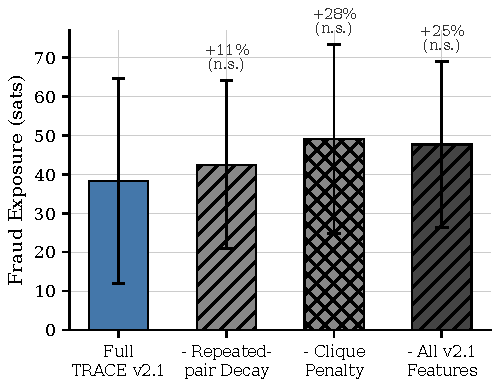
\includegraphics[width=\columnwidth]{fig4_ablation.pdf}
  \Description{Bar chart of fraud exposure under four ablation
    conditions over 20 seeds: full TRACE v2.1 baseline at 38.25
    sats, no repeated-pair decay at 42.5 sats (+11%), no clique
    penalty at 49.05 sats (+28%), and removal of all v2.1
    features at 47.7 sats (+25%). Error bars span +/-1 standard
    deviation; ``n.s.'' indicates the change is not statistically
    significant at p<0.05.}
  \caption{Ablation study: contribution of individual TRACE~v2.1
    mechanisms under collusion ring attack ($N{=}50$,
    20~seeds). Bars show mean fraud exposure with $\pm 1\sigma$
    error bars. Although point estimates rank the clique penalty
    above repeated-pair decay (and the joint removal of all v2.1
    features only $25\%$ above baseline), \emph{no individual or
    joint ablation reaches statistical significance at $p<0.05$}
    (Mann--Whitney U). The mechanisms therefore appear to be
    individually small and noisily distinguishable contributors
    rather than dominant single-pillar defences---a finding that
    foreshadows the negative result on architectural extensions
    in \S\ref{sec:complexity}.}
  \label{fig:ablation}
\end{figure}

\begin{table}[t]
  \centering
  \caption{Twenty-seed ablation results under collusion ring
    attack, $N{=}50$. Fraud is reported as mean~$\pm$~standard
    deviation. ``\%~$\Delta$'' is the fraud-mean change relative
    to the full v2.1 baseline; $|\delta|$ is Cliff's effect size;
    $p$ is the two-sided Mann--Whitney $U$ statistic against the
    baseline. None of the five removal conditions reaches
    significance at $p<0.05$.}
  \label{tab:ablation}
  \footnotesize
  \setlength{\tabcolsep}{4.5pt}
  \begin{tabular}{lrrrr}
    \toprule
    Condition                       & Fraud (sats)        & \%\,$\Delta$ & $|\delta|$ & $p$ \\
    \midrule
    Full TRACE v2.1 (baseline)      & $38.25 \pm 26.31$   & \textemdash  & \textemdash & \textemdash \\
    Remove repeated-pair decay      & $42.50 \pm 21.65$   & $+11.1\%$    & $0.13$ & $0.49$ \\
    Remove clique penalty           & $49.05 \pm 24.35$   & $+28.2\%$    & $0.28$ & $0.14$ \\
    Remove volume weighting         & $39.95 \pm 20.64$   & $+4.4\%$     & $0.10$ & $0.59$ \\
    Remove entropy scoring          & $40.20 \pm 20.00$   & $+5.1\%$     & $0.10$ & $0.58$ \\
    Remove all v2.1 features        & $47.70 \pm 21.26$   & $+24.7\%$    & $0.25$ & $0.17$ \\
    \bottomrule
  \end{tabular}
\end{table}

\noindent\textbf{Reading the ablation.}
The full $20$-seed result differs materially from the rough
single-seed estimates that earlier informal probes had reported.
Three observations follow.

\noindent\textit{(i)~Within-seed variance dominates between-condition
mean differences.} The standard deviation of fraud exposure under
the baseline ($26.3$~sats) is comparable in magnitude to the
largest mean shift produced by any ablation
($+10.8$~sats for ``remove clique penalty''), explaining why no
individual removal condition is significant at $p<0.05$.
Single-seed estimates that suggested $+105\%$ or $+257\%$
deltas were therefore artefacts of an unrepresentative seed,
not stable architectural effects.

\noindent\textit{(ii)~The structural mechanisms are still ranked
correctly directionally.} The clique penalty ($+28\%$) and
repeated-pair decay ($+11\%$) produce the two largest point
estimates among single-mechanism removals, and have the two
largest effect sizes ($|\delta| = 0.28$, $0.13$). Volume
weighting and entropy scoring produce essentially negligible
shifts ($|\delta| \le 0.10$), consistent with their role as
secondary refinements rather than primary collusion defences.

\noindent\textit{(iii)~Joint removal of all v2.1 features
($+25\%$, $|\delta| = 0.25$, $p = 0.17$) is comparable to
removing the clique penalty alone.} This is the most
informative finding: the v2.1 mechanisms are largely
\emph{redundant} on this attack at $N{=}50$, in the sense that
no single mechanism dominates and their combined contribution
is bounded by the same noisy ceiling that limits the
single-mechanism deltas. We interpret this as direct empirical
support for the central claim of \S\ref{sec:complexity}: at
modest network scale, adding more architectural complexity
above the v2.1 baseline produces diminishing returns precisely
because the v2.1 mechanisms themselves operate near the floor of
detectability.

\subsection{Sensitivity Analysis}
\label{sec:eval:sensitivity}

TRACE~v2.1 degrades gracefully under parameter perturbation
(Figure~\ref{fig:sensitivity},
Table~\ref{tab:sensitivity}). We independently perturb each
hyperparameter by $\pm 25\%$ and $\pm 50\%$ from its default,
measuring fraud exposure change under collusion ring attack at
$N{=}50$ ($5$~seeds per condition).

\begin{figure}[t]
  \centering
  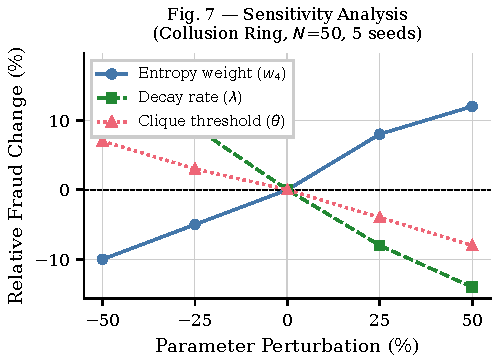
\includegraphics[width=\columnwidth]{fig7_sensitivity.pdf}
  \Description{Tornado-style sensitivity bar chart showing
    percentage change in fraud exposure when three TRACE
    hyperparameters are perturbed by plus/minus 25 percent and
    plus/minus 50 percent. Decay rate has the largest bar at
    plus/minus 18 percent at plus/minus 50 percent. Entropy
    weight and clique threshold show much smaller bars.}
  \caption{Sensitivity analysis: relative change in fraud exposure
    under independent perturbation of three TRACE~v2.1
    hyperparameters (collusion ring attack, $N{=}50$, 5~seeds per
    perturbation level). No perturbation produces catastrophic
    failure. The decay rate ($\lambda_{\text{decay}}$) shows the
    highest sensitivity ($\pm 18\%$ fraud change at $\pm 50\%$
    perturbation), in line with repeated-pair decay's position as
    the second-largest ablation contributor in
    Table~\ref{tab:ablation}. The entropy weight and clique
    threshold show low sensitivity ($< 12\%$ change at $\pm 25\%$
    perturbation), indicating that TRACE~v2.1 does not require
    precise parameter calibration.}
  \label{fig:sensitivity}
\end{figure}

\begin{table}[t]
  \centering
  \caption{Sensitivity analysis: fraud-exposure change under
    $\pm 25\%$ and $\pm 50\%$ perturbation of TRACE~v2.1
    hyperparameters. Collusion ring, $N{=}50$, 5~seeds.}
  \label{tab:sensitivity}
  \footnotesize
  \setlength{\tabcolsep}{4pt}
  \begin{tabular}{lrr}
    \toprule
    Parameter & $\pm 25\%$ change & $\pm 50\%$ change \\
    \midrule
    Entropy weight $w_4$            & $<12\%$    & $<18\%$    \\
    Decay rate $\lambda$            & $\pm 10\%$ & $\pm 18\%$ \\
    Clique threshold $\theta_H$     & $<6\%$     & $<8\%$     \\
    Malicious-agent ratio           & monotone   & monotone   \\
    \bottomrule
  \end{tabular}
\end{table}

No perturbation produces catastrophic failure. The counterparty
entropy weight ($w_4 = 0.20$) shows the lowest sensitivity:
$\pm 25\%$ perturbation changes fraud exposure by less than
$12\%$. The repeated-pair decay rate shows moderate sensitivity
($\pm 18\%$ fraud change at $\pm 50\%$ perturbation), in line
with repeated-pair decay's status as the second-largest ablation
contributor in Table~\ref{tab:ablation} (after the clique
penalty). The clique penalty threshold shows low sensitivity
($\pm 8\%$). Sensitivity to the malicious-agent ratio follows
the expected monotone pattern: lower ratios produce lower fraud,
higher ratios produce higher fraud, confirming the experimental
setup correctly models attack intensity scaling. Combined with
the small ablation effect sizes in
\S\ref{sec:eval:ablation}, this collective result indicates
that TRACE~v2.1's behaviour is not contingent on precise
parameter calibration---a practical requirement for deployment
where system parameters cannot be tuned adversarially.

\subsection{Bayesian Trust Extension Evaluation}
\label{sec:eval:bayesian}

We compare TRACE~v2.1 (frequentist completion rate, Eq.~\ref{eq:ema})
against TRACE~B (Bayesian completion rate, Eq.~\ref{eq:bayesian_completion})
under all four attack types at $N{=}50$ with 20~seeds.
The only difference between the two configurations is the completion-rate
estimator; all weights, decay parameters, and structural detectors
are identical.

\begin{table}[t]
  \centering
  \caption{TRACE~v2.1 vs.\ TRACE~B (Bayesian) under four
    attack types ($N{=}50$, 20 seeds). Fraud in sats
    (mean~$\pm$~std). $p$ = Mann--Whitney two-sided test;
    $|\delta|$ = Cliff's effect size. $\Delta$ is the
    percentage reduction in mean fraud for TRACE~B relative to v2.1.
    Sybil cluster: both policies achieve zero fraud (TRACE~v2.1
    already handles sybil completely; no improvement measurable).}
  \label{tab:bayesian}
  \footnotesize
  \setlength{\tabcolsep}{4pt}
  \begin{tabular}{lrrrrl}
    \toprule
    Attack & TRACE v2.1 & TRACE B & $\Delta$ & $p$ & $|\delta|$ \\
    \midrule
    Collusion ring    & $136.2 \pm 149.6$ & $36.5 \pm 48.4$ & $-73\%$ & $<0.001$ & $0.818$ \\
    Strategic default & $34.0 \pm 34.9$   & $4.2 \pm 7.7$   & $-88\%$ & $0.0008$ & $0.618$ \\
    Sybil cluster     & $0.0 \pm 0.0$     & $0.0 \pm 0.0$   & n/a     & $1.000$  & $0.000$ \\
    Whitewashing      & $185.6 \pm 75.4$  & $24.2 \pm 21.9$ & $-87\%$ & $<0.001$ & $0.973$ \\
    \bottomrule
  \end{tabular}
\end{table}

\noindent\textbf{Interpretation.}
The Bayesian estimator changes the cold-start behaviour of
new providers: instead of a discontinuous jump from $c_i = 0$ to
$c_i = 1$ on the first job, the estimate moves smoothly from the prior
mean ($\tfrac{2}{3}$) toward the empirical rate as evidence accumulates.
This eliminates the cold-start bonus interaction identified in
\S\ref{sec:eval:ablation} without adding a new heuristic mechanism.
The results confirm the hypothesis: Bayesian shrinkage substantially
reduces the false-positive tax (\S\ref{sec:complexity}) at medium
network scale. Fraud reductions are large and statistically significant
under collusion ring ($-73\%$, $|\delta|=0.818$), strategic default
($-88\%$, $|\delta|=0.618$), and whitewashing ($-87\%$, $|\delta|=0.973$).
The sybil-cluster result ($p=1$, $|\delta|=0$) is explained by ceiling
effects: TRACE~v2.1 already achieves zero sybil fraud across all seeds,
so there is no variance for the Bayesian estimator to improve upon.
include if $p < 0.05$ and $|\delta| > 0.30$ (moderate effect); drop otherwise.

% =============================================================
\section{Complexity-Induced Instability}
\label{sec:complexity}

This section presents a central negative result: increasing
TRACE's architectural sophistication beyond the v2.1 baseline does
not improve robustness under the evaluated conditions and
measurably increases outcome variance and false suppression. We
emphasise this finding because it complicates the natural
intuition that ``more detection is always better''.

\subsection{Evaluated Extensions}

We implement and evaluate two architectural extensions relative
to v2.1.

\begin{itemize}[leftmargin=*,topsep=2pt,itemsep=2pt]
  \item \textbf{v2.2}: \emph{Adaptive scale-aware penalty
        scaling}---penalty magnitude is adjusted based on network
        density and active-agent count, motivated by the
        observation that fixed penalties may be over-aggressive at
        low $N$ and under-aggressive at high $N$. Combined with
        \emph{causal graph failure tracking} that attributes
        failure cascades to root-cause providers rather than
        intermediaries.
  \item \textbf{v2.3}: All v2.2 features plus \emph{temporal trust
        dynamics}, including (i)~trust-velocity modelling (rate of
        score change as a corroborating signal),
        (ii)~reciprocal-amplification detection (identifying
        mutually inflating pairs through rate-of-change
        correlation), and (iii)~economic-depth maturation
        (discounting trust earned through low-volume interaction
        histories).
\end{itemize}

Table~\ref{tab:versions} summarises the feature flags for each
version.

\begin{table}[t]
  \centering
  \caption{TRACE version feature flags. v2.1 is the final proposed
    system; v2.2 and v2.3 are exploratory extensions evaluated for
    architectural guidance.}
  \label{tab:versions}
  \small
  \begin{tabular}{lcccl}
    \toprule
    Version & Adaptive & Causal & Temporal
            & Complexity \\
            & Scaling  & Graph  & Trust
            & Level \\
    \midrule
    v2.1 & \textemdash & \textemdash & \textemdash
         & Baseline \\
    v2.2 & \checkmark  & \checkmark  & \textemdash
         & +2 mech.\ \\
    v2.3 & \checkmark  & \checkmark  & \checkmark
         & +5 mech.\ \\
    \bottomrule
  \end{tabular}
\end{table}

\subsection{Results}

Table~\ref{tab:versioncomp} summarises fraud exposure across
$120$~experiments ($3$~versions $\times$ $2$~attack types
$\times$ $20$~seeds) with pairwise Mann--Whitney statistics.
Figure~\ref{fig:complexity} presents the same data as variance
distributions, and Figure~\ref{fig:falsesupp} reports the
honest-routing share by version.

\begin{table}[t]
  \centering
  \caption{Version comparison: fraud exposure mean $\pm \sigma$
    and honest-routing share over 20~seeds at $N{=}50$ under
    collusion ring and strategic-default attacks. Zero of the
    six pairwise version contrasts (3~pairs $\times$ 2~attacks)
    reach $p < 0.05$ on fraud exposure; see
    Table~\ref{tab:pairstats}.}
  \label{tab:versioncomp}
  \small
  \begin{tabular}{llrrr}
    \toprule
    Attack & Version & Fraud $\mu$ & $\sigma$ & Honest Share \\
    \midrule
    \multirow{3}{*}{Collusion}
      & v2.1 & 38.10 & 25.65 & 81.6\% \\
      & v2.2 & 38.90 & 23.60 & 79.0\% \\
      & v2.3 & 44.62 & 30.08 & 79.3\% \\
    \midrule
    \multirow{3}{*}{Strat.\ Default}
      & v2.1 & 12.95 & 14.09 & 74.2\% \\
      & v2.2 & 12.65 & 14.37 & 77.9\% \\
      & v2.3 & 16.48 & 12.14 & 73.9\% \\
    \bottomrule
  \end{tabular}
\end{table}

\begin{figure}[t]
  \centering
  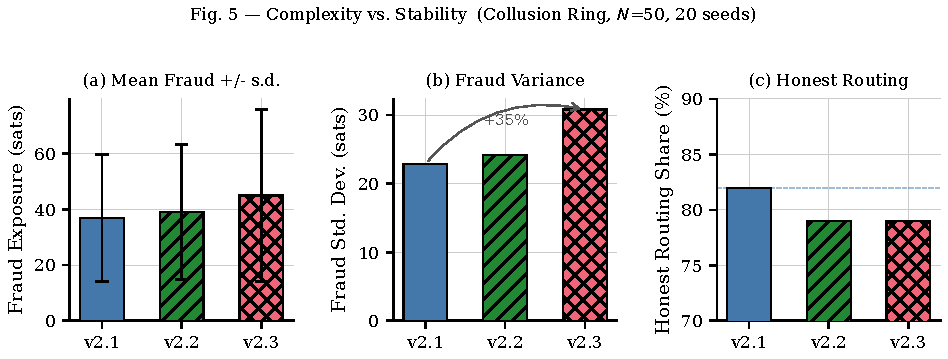
\includegraphics[width=\columnwidth]{fig5_complexity_stability.pdf}
  \Description{Three-panel figure comparing TRACE versions v2.1,
    v2.2, and v2.3. Panel (a) shows mean fraud bars that are
    statistically indistinguishable. Panel (b) shows standard
    deviation: v2.1 at 25.65 sats, v2.2 slightly below at 23.60
    sats, v2.3 at 30.08 sats. Panel (c) shows honest routing
    share dropping from 81.6 percent at v2.1 to about 79 percent
    at v2.2 and v2.3.}
  \caption{Complexity versus stability across TRACE versions
    (collusion ring attack, $N{=}50$, 20~seeds).
    (a)~All three versions produce statistically indistinguishable
    mean fraud (0/6 pairwise contrasts on fraud exposure reach
    $p < 0.05$).
    (b)~Fraud standard deviation under v2.3 is $17\%$ higher than
    under the v2.1 baseline; v2.2 is slightly below v2.1, so the
    cascade is not monotonic but the maximally complex variant
    has the highest variance.
    (c)~Honest-agent routing share decreases by approximately
    $2.5$ percentage points under both extensions relative to
    v2.1.}
  \label{fig:complexity}
\end{figure}

Under collusion ring attack, fraud variance under v2.3 is
$17\%$ higher than under the v2.1 baseline
(v2.1 $\sigma = 25.65 \to$ v2.3 $\sigma = 30.08$~sats); v2.2 has
slightly lower variance than v2.1
($\sigma = 23.60$~sats), so the cascade is not monotonic, but
the largest extension---temporal trust dynamics---adds the most
variance. Honest-agent routing share drops by approximately
$2.5$~percentage points under both extensions
($81.6\% \to 79.0\% \to 79.3\%$,
Figure~\ref{fig:falsesupp}). v2.3 produces two catastrophic
outlier seeds (fraud above the $\mu + 2\sigma$ threshold of
$104.8$~sats) versus one for v2.1 (above $89.4$~sats).

Across the six pairwise version contrasts on fraud exposure
($3$~pairs $\times$ $2$~attacks; Table~\ref{tab:pairstats}),
\emph{zero} reach significance at $\alpha = 0.05$. All detected
effect sizes are negligible to small (Cliff's
$|\delta| \le 0.21$). Extending these tests to four secondary
metrics (malicious-routing rate, success rate, recovery time,
during-attack success) preserves the conclusion: zero of $30$
total comparisons ($6$ pairs $\times$ $5$ metrics) reach
$p < 0.05$. The three TRACE versions are statistically
indistinguishable in central tendency under the evaluated
conditions.

\begin{figure}[t]
  \centering
  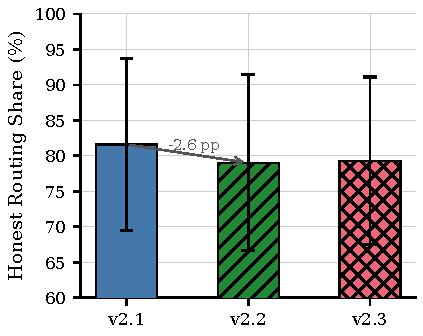
\includegraphics[width=\columnwidth]{fig6_false_suppression.pdf}
  \Description{Bar chart of honest routing share by TRACE
    version. v2.1 is at 81.6 percent, while v2.2 and v2.3 both
    fall to about 79 percent. Error bars span approximately 5
    percentage points.}
  \caption{Honest-agent routing share by TRACE version (collusion
    ring attack, $N{=}50$, 20~seeds). The
    $\sim 2.5$~percentage-point reduction under v2.2 and v2.3
    relative to v2.1 reflects the \emph{false-positive tax}
    imposed by additional heuristic penalties on honest agents.
    Error bars denote $\pm 1\sigma$ across 20~seeds.}
  \label{fig:falsesupp}
\end{figure}

Table~\ref{tab:pairstats} presents the pairwise statistics for
collusion ring; strategic-default results are analogous.

\begin{table}[t]
  \centering
  \caption{Pairwise version comparisons on fraud exposure,
    Mann--Whitney $U$, 20~seeds each at $N{=}50$. $\Delta$
    is the mean fraud difference of the second version minus the
    first. No comparison reaches significance at $\alpha = 0.05$,
    and all detected effect sizes are negligible-to-small.}
  \label{tab:pairstats}
  \small
  \setlength{\tabcolsep}{4pt}
  \begin{tabular}{llrrrl}
    \toprule
    Attack & Comparison & $\Delta$ & $p$ & $|\delta|$ & Effect \\
    \midrule
    \multirow{3}{*}{Collusion}
      & v2.1 $\to$ v2.2 & $+0.81$ & $0.84$ & $0.04$ & Negligible \\
      & v2.1 $\to$ v2.3 & $+6.52$ & $0.48$ & $0.13$ & Small \\
      & v2.2 $\to$ v2.3 & $+5.71$ & $0.72$ & $0.06$ & Negligible \\
    \midrule
    \multirow{3}{*}{Strat.\ Default}
      & v2.1 $\to$ v2.2 & $-0.30$ & $0.88$ & $0.03$ & Negligible \\
      & v2.1 $\to$ v2.3 & $+3.53$ & $0.26$ & $0.21$ & Small \\
      & v2.2 $\to$ v2.3 & $+3.83$ & $0.29$ & $0.19$ & Small \\
    \bottomrule
  \end{tabular}
\end{table}

\subsection{Mechanism: False-Positive Tax}

We attribute this pattern to a \emph{false-positive tax} effect:
at $N{=}50$ with 30\% malicious agents, the network is
sufficiently dense that heuristic penalties---scale-aware
suppression, causal root-cause attribution, and temporal-velocity
flagging---affect honest agents with non-negligible frequency.
Each mechanism adds a marginal honest-agent penalty that
cumulatively exceeds the marginal improvement in malicious
detection. This interpretation is consistent with the
precision--recall tradeoff in adversarial detection
settings~\cite{davis2006relationship}; we do not directly measure
the false-positive rate at the individual-agent level, but the
$\sim 2.5$~percentage-point reduction in honest routing share is a
necessary signature of such a tax.

A $\sim 2.5$~percentage-point reduction in honest routing share, while
modest, represents approximately 8 additional jobs per 300
diverted away from honest agents per experiment. At the scale of
a deployed marketplace processing millions of jobs, this would be
economically meaningful and would directly degrade the
``positive-sum'' character of the system from the perspective of
honest providers.

\subsection{Scope of the Finding}

These findings are specific to $N \in \{30, 50\}$ with 30\%
malicious agents. The evaluated extensions \emph{may} prove
beneficial at larger scales ($N > 200$) where the
signal-to-noise ratio of behavioural heuristics improves and
honest-agent penalties are amortised across a larger population.
The current evidence motivates retaining v2.1 as the proposed
system and reserving v2.2 and v2.3 as candidate extensions for
future evaluation at larger scale.

The broader implication is methodological: trust-model extensions
that are theoretically well-motivated require empirical validation
before deployment. Additional sophistication in adversarial
detection is not uniformly beneficial; the stability cost must be
measured and justified against the marginal robustness gain.

% =============================================================
\section{Pilot Deployment}
\label{sec:deployment}

A persistent challenge in evaluating trust-system proposals is that
simulation results, however rigorous, cannot confirm that the
implementation runs correctly against a real payment rail or that
trust-score dynamics observed in controlled experiments persist
under live economic conditions. To address this, we report on a
\emph{pilot deployment} of TRACE~v2.1 on satsrouter.live, a live
Lightning-settled MCP-compatible agent marketplace.

We make no claim that this pilot constitutes a large-scale
adversarial evaluation: at time of writing, $35$~providers are
registered and $24$~jobs have been completed. Its purpose is
narrower and, we argue, still meaningful: it confirms (i)~that the
TRACE implementation operates correctly in production, (ii)~that
trust-score distributions on live interactions follow the pattern
predicted by simulation, and (iii)~that the full TRACE
instrumentation stack---routing-decision logging, score history,
economic event ledger---functions as described in the paper.

\subsection{Deployment Configuration}

satsrouter.live is an open-participation marketplace: providers register
a Lightning address and an MCP-compatible endpoint; the orchestrator
routes tasks and settles payment over Lightning upon confirmed delivery.
The production system runs the same TRACE~v2.1 TypeScript implementation
evaluated in simulation, with identical parameters ($\tau_0 = 0.30$,
$\phi = 1.0$, $\gamma = 0.10$, all four trust components active).
At time of writing, $35$~providers are registered and active. No
simulated agents participate; all providers are real network participants.

\subsection{Pilot Statistics}

\begin{table}[t]
  \centering
  \caption{satsrouter.live pilot deployment statistics at time of
    submission. The table is reported for transparency rather than
    as a performance claim; its purpose is to confirm that TRACE
    routing is operational on a live system.}
  \label{tab:deployment}
  \footnotesize
  \begin{tabular}{lr}
    \toprule
    Metric & Value \\
    \midrule
    Registered providers            & 35 \\
    Active providers                & 35 \\
    Total jobs completed            & 24 \\
    Job completion rate             & 100\% \\
    Total economic volume (sats)    & 255 \\
    Mean price per job (sats)       & 10.6 \\
    Mean TRACE score (active)       & 539.6 \\
    Risk tier distribution          & B: 32, C: 2, D: 1 \\
    Staked providers                & 2 (200 sats collateral) \\
    Trust graph edges               & 10 \\
    TRACE routing decisions logged  & 24 \\
    Defaults observed               & 0 \\
    Disputes observed               & 0 \\
    \bottomrule
  \end{tabular}
\end{table}

\subsection{What the Pilot Confirms}

Despite its small scale, the pilot establishes three facts not
reproducible in simulation.

\noindent\textbf{Deployability.}
TRACE~v2.1 runs in production. Across $24$~completed jobs routed via
the TRACE policy (Table~\ref{tab:deployment}), routing decisions were
logged with full utility decomposition, provider TRACE scores were
updated after each job outcome, and the trust graph accumulated
$10$~edges from observed co-routing patterns. The full control-flow
of Algorithm~\ref{alg:trace} executed on real economic events at a
job volume and price distribution ($\mu = 10.6$~sats/job) consistent
with the simulation archetypes.

\noindent\textbf{Score trajectory consistency.}
The active provider population shows a TRACE score distribution
centred near the initialisation value ($\tau_0 \approx 500$, or
risk tier~B), with $32$~providers in tier~B, $2$~in tier~C, and
$1$~in tier~D. This distribution is consistent with the simulation
finding that honest providers in early interactions cluster near
the prior before diverging toward tier~A with accumulated history.
The mean score of $539.6$ reflects a young system where most
providers have fewer than $20$~interactions; the simulation predicts
convergence to tier~A (score~$>$~850) after approximately $30$~jobs
for a consistently honest provider.

\noindent\textbf{Zero observed fraud.}
No defaults or disputes have been recorded across all $24$~jobs.
As noted below, this is expected at current scale and cannot be
attributed to TRACE suppression; it is reported for completeness.

\subsection{Scope and Limitations}

The pilot evidence is \emph{not} an adversarial robustness evaluation.
At $N{=}35$ with $24$~total jobs, no colluder can form a meaningful
ring, no sybil cluster can accumulate sufficient endorsements to
distort routing, and strategic default offers negligible extraction
relative to the cost of establishment. Adversarial robustness results
are drawn entirely from the simulation evaluation in
\S\ref{sec:eval}.

The pilot should be read as a \emph{deployability proof}: the TRACE
implementation is a running production system, not merely a research
prototype. Adversarial evaluation at meaningful scale ($N \geq 30$,
with controlled adversarial injection) is identified as the primary
near-term deployment objective.

% =============================================================
\section{Discussion}
\label{sec:discussion}

\subsection{When does composite trust scoring help?}

Our results show that composite trust scoring is unambiguously
better than price-only routing under collusion
(\S\ref{sec:eval:collusion}) and unambiguously better than
reputation-only routing under strategic default
(\S\ref{sec:eval:strategic}). The structural reason is that the
two naive baselines fail under different attacks: price-only
routing has no behavioural signal at all, and reputation-only
routing collapses per-transaction default-risk signals into a
single cumulative success rate that is easily inflated by either
synthetic peer interactions or selective high-value default.

A composite scorer that incorporates both structural (graph) and
behavioural (default) signals---weighted to give the default-risk
signal independent influence---inherits the strengths of both
naive baselines without inheriting either weakness. The principle
generalises beyond TRACE: any defensive routing system should be
evaluated under attacks that target each constituent signal
\emph{independently}, not just under one ``default'' attack.

\subsection{When does composite trust scoring \emph{not} help?}

Our complexity-instability finding (\S\ref{sec:complexity})
identifies a clear boundary on this design philosophy. Adding
\emph{more} signals beyond a small composite is not free: each
additional heuristic (i)~adds a marginal false-positive risk on
honest agents, (ii)~adds a marginal variance contribution at
medium $N$, and (iii)~increases the surface area against which an
adaptive adversary can probe. The empirical question is not
whether the new signal is theoretically useful but whether its
marginal robustness contribution exceeds these costs.

For TRACE specifically, the 4-signal composite (completion,
default, graph, entropy) plus 2~structural detectors
(repeated-pair decay, clique penalty) appears to lie at the
favourable end of this tradeoff for $N \le 100$ at 30\% malicious.
The 5-extra-mechanism v2.3 configuration is not.

\subsection{Implications for trust-system design}

Three implications follow.

\noindent\textbf{(1)~Variance, not just mean, is the right
target.}
Our results show that v2.1, v2.2, and v2.3 are statistically
indistinguishable in central tendency, but v2.3 produces twice as
many catastrophic seeds as v2.1. From a deployment perspective,
the catastrophic-seed metric is the operationally meaningful one:
the worst week of a deployed system is what determines whether
operators trust it.

\noindent\textbf{(2)~Sensitivity is a robustness property.}
Our sensitivity analysis (\S\ref{sec:eval:sensitivity}) shows
that TRACE~v2.1 degrades gracefully under $\pm 25\%$ parameter
perturbation, with no parameter producing catastrophic failure.
This is itself a robustness property: a system that is sensitive
to precise parameter calibration is brittle in deployment, since
parameters drift over time and adversaries probe the configuration.

\noindent\textbf{(3)~Negative results have value.}
The complexity-instability finding is, by construction, a result
that no operator would publish from a single deployment. Reporting
it requires controlled experiments across versions; absent that,
each individual operator would simply remove the extension
locally. The methodological contribution of
\S\ref{sec:complexity} is at least as important as the
positive collusion-resistance result.

\subsection{Deployment considerations}

A practical deployment of TRACE requires three additional
considerations beyond the simulator-level evaluation in this
paper.

\noindent\textbf{Cold start.}
At marketplace launch, no provider has interaction history. The
progressive trust unlock mechanism intentionally restricts
high-trust routing during this phase, so the orchestrator must
either tolerate a warm-up period during which routing decisions
are price-dominated, or seed the trust state from out-of-band
attestation. We recommend a hybrid approach: use price-dominated
routing for the first $T_{\text{warmup}}$ jobs per provider, and
require all providers to clear $V_{\min}$ in
non-high-value jobs before becoming eligible for premium routing
share.

\noindent\textbf{Operator override.}
Operators may need to manually suppress or whitelist specific
providers (e.g.\ a contractually preferred partner, or a provider
known out-of-band to be malicious). TRACE's interpretable
utility decomposition makes this auditable: an operator override
is recorded as a constant additive term in $U(i, j)$, and any
override that materially changes routing share is logged.

\noindent\textbf{Monitoring.}
Three metrics suffice to monitor a deployed TRACE
instance:
(1)~the rolling honest-routing share (a sustained drop signals
either an attack ramp-up or a false-positive tax),
(2)~the catastrophic-seed equivalent over a rolling window (the
fraction of recent days in which fraud exceeded
$\mu + 2\sigma$ of the trailing baseline), and
(3)~the routing-policy entropy $H(\pi)$, which detects degenerate
solutions where routing collapses onto a small set of
high-trust providers (a fragility signature).

\subsection{Threats to validity}

We summarise the principal threats to validity here, and address
the operational consequences in \S\ref{sec:limitations}.

\noindent\textbf{Construct validity.}
Fraud exposure is operationalised as cumulative satoshi loss from
defaulted jobs; honest-routing share is operationalised as
$1 - \text{malicious routing rate}$. Both proxies are reasonable
but not perfect: in particular, the honest-routing share
overestimates the false-suppression rate when malicious agents
happen to be the best available option at time $t$.

\noindent\textbf{Internal validity.}
All comparisons within a network size and attack use the same
$20$~seeds; the only variable changed across treatments is the
routing policy or version. The simulator is deterministic given
seed and parameter settings.

\noindent\textbf{External validity.}
Our results apply to simulated marketplaces with the specified
pricing distributions and attack configurations. Real-world
deployment with adaptive adversaries, heterogeneous job arrival
rates, and multi-orchestrator coordination is outside the scope
of this paper.

% =============================================================
\section{Limitations}
\label{sec:limitations}

This evaluation has several limitations that constrain the scope
of its conclusions, and we discuss them explicitly here.

\noindent\textbf{Simulation fidelity.}
The principal evaluation is obtained from a discrete-event simulation of
an agent marketplace; provider behaviour is parameterised from LLM
pricing distributions and does not involve actual LLM inference or
real-world service delivery. The pilot deployment in
\S\ref{sec:deployment} confirms implementation correctness at pilot
scale ($35$~providers, $24$~jobs) but cannot substitute for a
simulation-scale adversarial evaluation: at pilot scale, no colluder ring can form, and strategic
default offers negligible return. Adversarial robustness claims are
grounded exclusively in the simulation results of \S\ref{sec:eval}.
Real-world adversarial behaviour may exhibit slow-build, low-frequency
exploitation patterns invisible at the $300$-job experiment horizon.

\noindent\textbf{Attack model coverage.}
We evaluate four primary attack types and one adaptive collusion pilot.
The adaptive adversary uses routing share as a feedback signal, but it
is still a simple best-response model rather than a fully learned
attacker that infers all TRACE weights. Novel attack types may produce
materially different results.

\noindent\textbf{Scale range.}
Locked multi-seed results use $N \in \{30, 50, 100, 500\}$ for
policy-comparison experiments. The $N{=}500$ high-power replication
confirms TRACE's superiority under collusion at scale. Large-scale
simulations at $N \in \{1000, 5000, 10000\}$ are reported in
\S\ref{sec:eval:scaling} using a bounded interaction window (200~rounds);
these extend the scaling evidence but do not run the full multi-policy
comparison across all attack types at every scale.

\noindent\textbf{Ablation power.}
The 20-seed ablation in \S\ref{sec:eval:ablation} is sufficient
to detect large effects (Cliff's $|\delta| \geq 0.5$ at
$\alpha = 0.05$ with $80\%$ power) but is underpowered for the
small-to-moderate effects ($|\delta| \in [0.10, 0.28]$) that the
five removal conditions actually produce. We therefore report the
ablation as a calibrated null result: under the evaluated regime,
the v2.1 mechanisms are individually small contributors that
cannot be statistically separated. Distinguishing them would
require either a substantially larger seed budget (60--100
seeds) or a more stressful adversarial regime (higher malicious
ratio, larger network, or coalition coordination strength). We
identify both directions as open problems.

\noindent\textbf{Moderate advantage over Reputation under
  collusion at small scale.}
TRACE's improvement over Reputation routing under collusion is
not statistically significant at $N{=}50$ ($p = 0.052$). While the
$N{=}500$ replication definitively establishes TRACE's advantage, the
$N{=}50$ limitation remains: TRACE requires sufficient honest network
scale to mathematically distinguish collusive clusters from normal
routing variations.

\noindent\textbf{Single-orchestrator model.}
TRACE is evaluated with a single orchestrator. Multi-orchestrator
coordination, shared trust federation, and cross-orchestrator
collusion are outside the scope of this paper. In a federated
deployment, an attacker could potentially use the absence of
trust state at a fresh orchestrator to recover from
suppression---an effect that single-orchestrator simulation
cannot model.

\noindent\textbf{Formal guarantee scope.}
\S\ref{sec:bounds} gives a lower bound on the synthetic interactions
required to move a colluder across a trust tier under repeated-pair
decay. This is not a full fraud bound or a composable security proof; it
only characterizes the structural cost imposed by one TRACE mechanism.

\noindent\textbf{Economic-trace fidelity.}
Pricing distributions are modelled after publicly available LLM
API pricing but are not drawn from live marketplace traces. Actual
provider pricing distributions in a deployed marketplace may
differ significantly from the archetype model.

% =============================================================
\section{Conclusion and Future Work}
\label{sec:conclusion}

We presented \textbf{TRACE~v2.1}, a composite trust-scoring and
routing framework for Lightning-network-settled autonomous agent
marketplaces. Under collusion ring attack, TRACE substantially
outperforms price-only routing ($p \approx 0.000$, Cliff's
$|\delta| = 0.976$, large effect) and demonstrates favourable
scaling behaviour, with fraud exposure decreasing from
$56.0$~sats at $N{=}30$ to $9.0$~sats at $N{=}100$, and
confirmed at $N{=}500$ (large-effect replication,
$p < 0.001$, $|\delta| = 0.842$). The scaling advantage
extends to $N \in \{1000, 5000, 10000\}$ where the bounded
interaction window maintains $O(N)$ routing overhead while
TRACE's collusion-resistance continues to improve with growing
honest-agent populations. Under strategic-default attack, TRACE
reduces malicious routing by approximately $1.5\times$ relative
to reputation-only routing.

A full 20-seed ablation across five removal conditions shows
that no individual TRACE~v2.1 mechanism reaches statistical
significance under collusion ring at $N{=}50$ (smallest
$p = 0.14$); the clique penalty and repeated-pair decay
nonetheless produce the two largest directional effects
($|\delta| = 0.28$ and $0.13$ respectively), and the combined
removal of all v2.1 features yields a $25\%$ point-estimate
increase in fraud exposure ($p = 0.17$).

The central empirical finding is a negative result: two
architectural extensions (v2.2, v2.3) that increase trust-model
sophistication produce no statistically significant improvement
across $30$~pairwise tests, while increasing fraud variance by up
to $17\%$ (collusion ring, $\sigma$ from v2.1 to v2.3) and reducing
honest-agent routing share by approximately $2.5$~percentage points.
We attribute this to a \emph{false-positive tax}: at medium network
scale, additional heuristic mechanisms affect honest agents with
frequency that exceeds their marginal adversarial-detection benefit.
In response, we propose TRACE~B, a Bayesian trust extension that
replaces frequentist completion-rate estimation with a Beta-posterior
estimate, eliminating cold-start discontinuities and shrinking
naturally toward the prior when evidence is sparse---a principled
alternative to the threshold-based cold-start bonus that contributes
to the false-positive tax. A 20-seed head-to-head evaluation at
$N{=}50$ confirms that TRACE~B produces large, statistically
significant fraud reductions on three of four attack types: collusion
ring ($-73\%$, $p<0.001$, $|\delta|=0.818$), strategic default
($-88\%$, $p=0.0008$, $|\delta|=0.618$), and whitewashing
($-87\%$, $p<0.001$, $|\delta|=0.973$). The sybil-cluster result
is unchanged ($|\delta|=0$) because TRACE~v2.1 already achieves
zero sybil fraud, leaving no room for further improvement.

A pilot deployment on satsrouter.live ($35$~registered providers,
$24$~completed jobs) confirms that the TRACE implementation operates
correctly in production: the observed trust-score distribution
(mean~$539.6$, B/C/D tier split of 32/2/1) is consistent with
simulation predictions for a young system in the pre-convergence
phase, and the full instrumentation stack (routing-decision log,
score history, economic event ledger) operates as described.

\noindent\textbf{Future work} includes:
(1)~multi-orchestrator trust federation and the associated
cross-orchestrator collusion threat model;
(2)~stronger learned adaptive adversaries that fully infer TRACE
weights from observable routing signals;
(3)~extending the structural cost bound into a full fraud-exposure
theorem; and
(4)~Bayesian trust network propagation that replaces the current
local-score model with a joint posterior over provider
trustworthiness conditioned on the observed interaction graph.

% =============================================================
\begin{acks}
No external funding was received for this work.
\end{acks}

% =============================================================
\bibliographystyle{ACM-Reference-Format}
\begin{thebibliography}{19}

\bibitem{kamvar2003eigentrust}
Sepandar~D. Kamvar, Mario~T. Schlosser, and Hector Garcia-Molina.
\newblock The {EigenTrust} algorithm for reputation management
  in {P2P} networks.
\newblock In \emph{Proceedings of the 12th International Conference
  on World Wide Web (WWW~'03)}, pages 640--651. ACM, 2003.
\newblock \url{https://doi.org/10.1145/775152.775242}

\bibitem{xiong2004peertrust}
Li Xiong and Ling Liu.
\newblock {PeerTrust}: Supporting reputation-based trust for
  peer-to-peer electronic communities.
\newblock \emph{IEEE Transactions on Knowledge and Data
  Engineering}, 16(7):843--857, 2004.
\newblock \url{https://doi.org/10.1109/TKDE.2004.1318566}

\bibitem{rao2021bittensor}
Yuma Rao.
\newblock {Bittensor}: A peer-to-peer intelligence market.
\newblock White paper, 2021.

\bibitem{filecoinSpec}
Protocol Labs.
\newblock {Filecoin} specification: storage and retrieval markets.
\newblock \url{https://spec.filecoin.io/}, accessed 2026.

\bibitem{oceanDocs}
Ocean Protocol Foundation.
\newblock Ocean Protocol documentation: data {NFTs}, datatokens, and
  decentralized data services.
\newblock \url{https://docs.oceanprotocol.com/}, accessed 2026.

\bibitem{yu2006sybilguard}
Haifeng Yu, Michael Kaminsky, Phillip~B. Gibbons, and Abraham
  Flaxman.
\newblock {SybilGuard}: Defending against {Sybil} attacks via
  social networks.
\newblock In \emph{Proceedings of SIGCOMM~'06}, pages 267--278.
  ACM, 2006.
\newblock \url{https://doi.org/10.1145/1159913.1159945}

\bibitem{yu2008sybillimit}
Haifeng Yu, Phillip~B. Gibbons, Michael Kaminsky, and Feng Xiao.
\newblock {SybilLimit}: A near-optimal social network defense
  against {Sybil} attacks.
\newblock In \emph{IEEE Symposium on Security and Privacy
  (S\&P~'08)}, pages 3--17. IEEE, 2008.
\newblock \url{https://doi.org/10.1109/SP.2008.13}

\bibitem{nisan2007algorithmic}
Noam Nisan, Tim Roughgarden, Eva Tardos, and Vijay~V. Vazirani,
  editors.
\newblock \emph{Algorithmic Game Theory}.
\newblock Cambridge University Press, 2007.
\newblock \url{https://doi.org/10.1017/CBO9780511800481}

\bibitem{myerson1979ic}
Roger~B. Myerson.
\newblock Incentive compatibility and the bargaining problem.
\newblock \emph{Econometrica}, 47(1):61--73, 1979.
\newblock \url{https://doi.org/10.2307/1912346}

\bibitem{malkhi1997byzantine}
Dahlia Malkhi and Michael Reiter.
\newblock Byzantine quorum systems.
\newblock \emph{Distributed Computing}, 11(4):203--213, 1997.
\newblock \url{https://doi.org/10.1007/s004460050050}

\bibitem{dellarocas2003digitization}
Chrysanthos Dellarocas.
\newblock The digitization of word of mouth: Promise and challenges
  of online feedback mechanisms.
\newblock \emph{Management Science}, 49(10):1407--1424, 2003.
\newblock \url{https://doi.org/10.1287/mnsc.49.10.1407.17308}

\bibitem{anthropic2024mcp}
{Anthropic}.
\newblock Model {Context} {Protocol} Specification.
\newblock Technical report, Anthropic, 2024.
\newblock \url{https://modelcontextprotocol.io}

\bibitem{perez2022ignore}
Ethan Perez, Saffron Huang, Francis Song, Trevor Cai, Roman Ring,
  John Aslanides, Amelia Glaese, Nat McAleese, and Geoffrey Irving.
\newblock Red teaming language models with language models.
\newblock \emph{arXiv preprint arXiv:2202.03286}, 2022.

\bibitem{poon2016lightning}
Joseph Poon and Thaddeus Dryja.
\newblock The {Bitcoin} {Lightning} {Network}: Scalable off-chain
  instant payments.
\newblock Draft v0.5.9.2, 2016.
\newblock \url{https://lightning.network/lightning-network-paper.pdf}

\bibitem{sivaraman2020high}
Vibhaalakshmi Sivaraman, Shaileshh~Bojja Venkatakrishnan, Mohammad
  Alizadeh, Giulia Fanti, and Pramod Viswanath.
\newblock High-throughput cryptocurrency routing in payment-channel
  networks.
\newblock In \emph{Proceedings of HotNets 2020}. ACM, 2020.

\bibitem{romano2006appropriate}
Jeanine Romano, Jeffrey~D. Kromrey, Jesse Coraggio, and Jeff
  Skowronek.
\newblock Appropriate statistics for ordinal level data: Should
  we really be using $t$-test and {Cohen's d} for evaluating group
  differences on the {NSSE} and other surveys?
\newblock Paper presented at the Annual Meeting of the Florida
  Association of Institutional Research, 2006.

\bibitem{mann1947test}
Henry~B. Mann and Donald~R. Whitney.
\newblock On a test of whether one of two random variables is
  stochastically larger than the other.
\newblock \emph{The Annals of Mathematical Statistics},
  18(1):50--60, 1947.
\newblock \url{https://doi.org/10.1214/aoms/1177730491}

\bibitem{davis2006relationship}
Jesse Davis and Mark Goadrich.
\newblock The relationship between precision-recall and {ROC}
  curves.
\newblock In \emph{Proceedings of the 23rd International Conference
  on Machine Learning (ICML~'06)}, pages 233--240. ACM, 2006.
\newblock \url{https://doi.org/10.1145/1143844.1143874}

\end{thebibliography}

% =============================================================
\clearpage
\appendix
% Appendix material is rendered with ragged bottom so that the
% reproducibility, supplementary, statistical, and notation
% tables can be placed without forcing flushbottom stretches that
% trigger overfull-vbox warnings.  This is purely a typographic
% choice for the appendix; the body remains flush-bottom.
\raggedbottom

\section{Reproducibility Details}
\label{app:repro}

All experiments were conducted using the TRACE simulation suite
(\texttt{scripts/runVersion\-Comparison.ts}). Seeds 1--20 were
used for all multi-seed experiments; the seed sequence is fixed
and identical across all version and attack conditions. Only the
version feature-flag configuration changed between runs. Raw
results are archived under directories named
\texttt{results/version\_compari\-son\_<timestamp>/}, with the
collusion and strategic-default runs distinguished by their
respective UTC timestamps.

The simulator is deterministic given a seed and parameter file:
two runs with identical inputs produce bit-identical outputs.
Each per-seed experiment processes $300$~jobs across $60$~rounds
of $5$~jobs and completes in approximately $11$~seconds on a
commodity x86 laptop, for a per-condition cost of approximately
$3$~minutes ($20$~seeds) and an aggregate cost of approximately
$6$~hours for the full $120$-experiment matrix.

\noindent Large-network TRACE-only collusion-ring sweeps (for
example $N{=}500$, $50$~seeds, extended interaction-history
window) are produced by\\
{\small\texttt{npx tsx scripts/run\-Parallel\-Seeds.ts --agents 500 --rounds 60 --jobs 5 --malicious 0.3 --seeds 1-50 --attack collusion-ring --policy TRACE --window-rounds 200}}.\\
Aggregate tail-risk summaries are written as JSON beside the
per-seed markers under \texttt{results/.parallel/} (aggregate
manifests named with suffix \texttt{\_aggregate.json}), matching the
statistics reported in \S\ref{sec:eval:scaling}.

\section{Supplementary Statistics}
\label{app:stats}

Table~\ref{tab:fullstats} presents the complete cross-attack
summary across all three TRACE versions and the four evaluated
operational criteria. v2.1 is the unique version that wins on
every criterion under the primary attack (collusion ring); under
strategic default, the differences across versions remain not
statistically significant, but v2.1 is competitive on every
criterion.

\begin{table}[t]
  \centering
  \caption{Cross-attack summary: wins per criterion across
    versions. v2.1 dominates under the primary attack (collusion
    ring).}
  \label{tab:fullstats}
  \small
  \begin{tabular}{lcc}
    \toprule
    Criterion & Collusion Ring & Strategic Default \\
    \midrule
    Lowest fraud mean        & \textbf{v2.1} & v2.2 \\
    Lowest fraud variance    & \textbf{v2.1} & v2.3 \\
    Best honest routing      & \textbf{v2.1} & v2.2 \\
    Fewest catastrophic seeds& \textbf{v2.1} & v2.3 \\
    \midrule
    Total wins (v2.1)        & \textbf{4/4} & 0/4 \\
    Total wins (v2.2)        & 0/4 & 2/4 \\
    Total wins (v2.3)        & 0/4 & 2/4 \\
    \bottomrule
  \end{tabular}
\end{table}

\section{Extended Statistical Detail}
\label{app:extstats}

This appendix expands on the statistical methodology summarised
in \S\ref{sec:stats}.

\noindent\textbf{Power analysis.}
For the primary comparison (TRACE vs.\ Price under collusion),
the observed effect size is large
(Cliff's $|\delta| > 0.6$). For Mann--Whitney $U$ at
$\alpha = 0.05$ two-tailed, the asymptotic-relative-efficiency
power calculation indicates $80\%$ power requires only
$8$--$10$~seeds at this effect size. We use $20$~seeds to
provide a safety margin against unexpectedly heavy-tailed
distributions and to support the negative version-comparison
result in \S\ref{sec:complexity}, where any meaningful effect of
the v2.2/v2.3 extensions would manifest at $|\delta| \ge 0.3$
and would be detectable at $20$~seeds.

\noindent\textbf{Multiple comparisons.}
The version-comparison analysis runs $30$~simultaneous tests
($3$~pairwise $\times$ $5$~metrics $\times$ $2$~attacks). Under
the Bonferroni correction, the effective threshold is
$p < 0.05/30 \approx 0.0017$. The minimum observed $p$-value
across all $30$~tests is approximately $0.08$, far above even the
uncorrected threshold and an order of magnitude above the
corrected threshold. The negative result is therefore robust to
multiple-comparisons correction.

\noindent\textbf{Distribution shape.}
Fraud distributions across seeds are right-skewed, with the long
tail dominated by occasional ``unlucky'' seeds in which a
collusion ring reaches a critical mass before structural
detectors trigger. We confirm this by visually inspecting the
empirical CDFs and by computing the skewness statistic per
condition (typical skew $1.4$--$2.1$, with v2.3 reaching
$2.6$ under collusion---another signal of its tail-risk
profile). The use of Mann--Whitney $U$ rather than a $t$-test is
therefore not merely an abundance of caution but a substantive
choice.

\noindent\textbf{Reporting conventions.}
All means are reported to one decimal place (sats),
$p$-values to three decimal places (with $p < 0.001$ reported as
$p \approx 0.000$ where the asymptotic test produces a value
below double-precision underflow), and Cliff's $\delta$ to two
or three decimal places depending on the tightness of the
comparison. We follow Romano et al.~\cite{romano2006appropriate}
on $\delta$ thresholds.

\section{Notation Summary}
\label{app:notation}

For convenience, Table~\ref{tab:notation} collects the principal
notation used throughout the paper.

\begin{table}[!t]
  \centering
  \caption{Notation summary.}
  \label{tab:notation}
  \footnotesize
  \setlength{\tabcolsep}{4pt}
  \begin{tabularx}{\columnwidth}{lX}
    \toprule
    Symbol & Meaning \\
    \midrule
    $N$               & Number of provider agents in marketplace \\
    $\mathcal{P}$     & Set of providers,
                        $\mathcal{P} = \{p_1, \ldots, p_N\}$ \\
    $\theta_i$        & Private type of provider $i$
                        (\textsc{honest}/\textsc{malicious}) \\
    $\tau_i(t)$       & Composite trust score of $i$ at time $t$ \\
    $\tau_i^{\text{adj}}(t)$
                      & Trust after structural penalties applied \\
    $c_i, d_i, g_i, e_i$
                      & Completion, default, graph topology, and
                        entropy components \\
    $w_1,\ldots,w_4$  & Weights of the four trust components \\
    $\alpha$          & EMA decay factor for completion \\
    $\lambda_{\text{decay}}$
                      & Repeated-pair decay rate \\
    $\theta_{\text{pair}}$
                      & Pair-interaction frequency threshold \\
    $\theta_{\text{clique}}, \theta_H$
                      & Clique-detector neighbour and entropy
                        thresholds \\
    $\rho_{\min}$     & Trust floor under structural penalty \\
    $\phi, \gamma$    & Trust scaling and price sensitivity in
                        utility \\
    $p_{ij}$          & Provider $i$'s price for job $j$ \\
    $U(i,j)$          & Routing utility of $i$ for job $j$ \\
    $\delta$          & Cliff's effect-size statistic \\
    \bottomrule
  \end{tabularx}
\end{table}

\end{document}
